\documentclass[a4paper, 11pt, onecolumn]{article} 

% arara: pdflatex 
% arara: bibtex
% arara: pdflatex
% arara: pdflatex
% arara: clean: {extensions: [ aux, bbl, out, toc, blg, thm ]}

\usepackage[doi, natbibapa]{apacite}

\usepackage{enumitem}
\usepackage[english]{babel}
%if french
%\frenchbsetup{StandardLists=true}

\usepackage[T1]{fontenc}
\usepackage[utf8]{inputenc}

\usepackage{lmodern}

\let\CheckCommand\providecommand
\usepackage{microtype}
\usepackage{hyperref}
%\usepackage[pagebackref=true]{hyperref}
%\renewcommand*{\backrefalt}[4]{#1}

\usepackage{lscape}
\usepackage{graphicx}
\usepackage{amssymb,amsmath}
\usepackage{url}
\usepackage{longtable}
\usepackage{tabu}
\usepackage{siunitx}                        
%\usepackage{threeparttable} 
\usepackage{array}
\usepackage{booktabs}

%\usepackage[french]{authblk}
%\DeclareCaptionFormat{twodot}{:}
\usepackage[font=small,skip=1em]{caption}


\usepackage{setspace}
\usepackage{fullpage}
\usepackage{eso-pic}

\usepackage[explicit, clearempty]{titlesec}
\usepackage[tableposition=top]{caption}
%\usepackage{titlesec}
\usepackage[a4paper]{geometry}

\usepackage{adjustbox}
\usepackage{rotating}
\usepackage{hvfloat}
\usepackage{wrapfig}
\usepackage{tfrupee}  
%\usepackage{multicol}

\usepackage{calc}

\usepackage{lettrine}
\usepackage{oldgerm}

\usepackage{fancyhdr}
\usepackage{lipsum}  
\usepackage{lastpage}

\usepackage{changepage}

% *****************************************************************
% Annexes
% *****************************************************************
%\usepackage[title, titletoc]{appendix}
\usepackage[toc,page]{appendix}
%\renewcommand\appendixtocname{Annexes}
%\renewcommand\appendixname{Annxes}
%\renewcommand\appendixpagename{Annexes}

% *****************************************************************
% Estout related things
% *****************************************************************
\newcommand{\sym}[1]{\rlap{#1}}

\let\estinput=\input% define a new input command so that we can still flatten the document

\newcommand{\estwide}[3]{
		\vspace{.75ex}{
			\begin{tabular*}
			{\textwidth}{@{\hskip\tabcolsep\extracolsep\fill}l*{#2}{#3}}
			\toprule
			\estinput{#1}
			\bottomrule
			\addlinespace[.75ex]
			\end{tabular*}
			}
		}	

\newcommand{\estauto}[3]{
		\vspace{.75ex}{
			\begin{tabular}{l*{#2}{#3}}
			\toprule
			\estinput{#1}
			\bottomrule
			\addlinespace[.75ex]
			\end{tabular}
			}
		}

% Allow line breaks with \\ in specialcells
	\newcommand{\specialcell}[2][c]{%
	\begin{tabular}[#1]{@{}c@{}}#2\end{tabular}}

% *****************************************************************
% Custom subcaptions
% *****************************************************************
% Note/Source/Text after Tables
\newcommand{\figtext}[1]{
	\vspace{-1.9ex}
	\captionsetup{justification=justified,font=footnotesize}
	\caption*{\hspace{6pt}\hangindent=1.5em #1}
	}
\newcommand{\fignote}[1]{\figtext{\emph{Note:~}~#1}}

\newcommand{\figsource}[1]{\figtext{\emph{Source:~}~#1}}

% Add significance note with \starnote
\newcommand{\starnote}{\figtext{* p < 0.1, ** p < 0.05, *** p < 0.01. Standard errors in parentheses.}}

% *****************************************************************
% siunitx
% *****************************************************************
\usepackage{siunitx} % centering in tables
	\sisetup{
		detect-mode,
		tight-spacing		= true,
		group-digits		= false ,
		input-signs		= ,
		input-symbols		= ( ) [ ] - + *,
		input-open-uncertainty	= ,
		input-close-uncertainty	= ,
		table-align-text-post	= false
        }

% *****************************************************************
% Sources
% *****************************************************************
\newcommand{\sourcetab}[1]{\vspace{-1em} \caption*{ \textbf{Source}: {#1}} }
\newcommand{\sourcefig}[1]{\vspace{-2em} \caption*{ \textbf{Source}: {#1}} }

\addto\captionsenglish{\renewcommand{\figurename}{\textbf{Figure}}}
\addto\captionsenglish{\renewcommand{\tablename}{\textbf{Table}}}


% *****************************************************************
% Abstract
% *****************************************************************
\let\abstractname\abstracteng

% *****************************************************************
% Hypothèses
% *****************************************************************
\usepackage{ntheorem}
\theoremseparator{:}
\newtheorem{hyp}{Hypothesis}

% \makeatletter
% \newcounter{subhyp} 
% \let\savedc@hyp\c@hyp
% \newenvironment{subhyp}
 % {%
  % \setcounter{subhyp}{0}%
  % \stepcounter{hyp}%
  % \edef\saved@hyp{\thehyp}% Save the current value of hyp
  % \let\c@hyp\c@subhyp     % Now hyp is subhyp
  % \renewcommand{\thehyp}{\saved@hyp\alph{hyp}}%
 % }
 % {}
% \newcommand{\normhyp}{%
  % \let\c@hyp\savedc@hyp % revert to the old one
  % \renewcommand\thehyp{\arabic{hyp}}%
% } 
% \makeatother

% *****************************************************************
% Tableaux
% *****************************************************************
\addto\captionsfrench{\def\tablename{\textsc{Table}}}

% *****************************************************************
% Bigcenter
% *****************************************************************
%%% ----------debut de bigcenter.sty--------------
 
%%% nouvel environnement bigcenter
%%% pour centrer sur toute la page (sans overfull)
 
%\newskip\@bigflushglue \@bigflushglue = -100pt plus 1fil
 
%\def\bigcenter{\trivlist \bigcentering\item\relax}
%\def\bigcentering{\let\\\@centercr\rightskip\@bigflushglue%
%\leftskip\@bigflushglue
%\parindent\z@\parfillskip\z@skip}
%\def\endbigcenter{\endtrivlist}
 
%%% ----------fin de bigcenter.sty--------------
%%%% fin macro %%%%
\makeatletter
\newskip\@bigflushglue \@bigflushglue = -100pt plus 1fil
\def\bigcenter{\trivlist \bigcentering\item\relax}
\def\bigcentering{\let\\\@centercr\rightskip\@bigflushglue%
\leftskip\@bigflushglue
\parindent\z@\parfillskip\z@skip}
\def\endbigcenter{\endtrivlist}
\makeatother

% *****************************************************************
% Lignes de code
% *****************************************************************
\usepackage{listings}
\lstset{ 
basicstyle=\scriptsize\ttfamily,
breaklines=true,
keywordstyle=\bf \color{blue},
commentstyle=\color[gray]{0.5},
stringstyle=\color{red},
showstringspaces=false,
numbers=left,
numberstyle=\tiny \bf \color{blue},
stepnumber=1,
numbersep=10pt,
firstnumber=1,
numberfirstline=true,
frame=leftline,
xleftmargin=0.5cm
}
 
% *****************************************************************
% Auteurs en bleu
% *****************************************************************
%\renewcommand{\citep}[1]{\textcolor{teal}{\citep{#1}}}
%\renewcommand{\cite}[1]{\textcolor{teal}{\cite{#1}}}
\usepackage{xcolor}
\usepackage{colortbl}

\hypersetup{colorlinks,linkcolor={red},citecolor={teal},urlcolor={blue}}
%\newcommand{\ypenser}[1]{\textcolor[purple]{#1}}
\newcommand{\ypenser}[1]{\textbf{\color{purple}--#1--}}

% *****************************************************************
% Mail
% *****************************************************************
\newcommand{\email}[1]{\href{mailto:#1}{\nolinkurl{#1}}}

% *****************************************************************
% Résumé et mots clés
% *****************************************************************
 \newenvironment{resab}[1]
{\begin{adjustwidth}{0cm}{0cm} \hangafter =1\par
    {\normalsize\bfseries #1\ \\ }\normalsize}
{\end{adjustwidth}\medskip}

 \newenvironment{keywords}
{\begin{adjustwidth}{0cm}{0cm} \hangafter =1\par
    {\normalsize\itshape Keywords:}~\normalsize}
{\end{adjustwidth}\medskip}

 \newenvironment{jelcodes}
{\begin{adjustwidth}{0cm}{0cm} \hangafter =1\par
    {\normalsize\itshape JEL Codes:}~\normalsize}
{\end{adjustwidth}\medskip}

% *****************************************************************
% Poete
% *****************************************************************
\newcommand{\attrib}[1]{%
\nopagebreak{\raggedleft\footnotesize #1\par}}

% *****************************************************************
% Stata
% *****************************************************************
\newcommand{\Stata}{%
\textsc{Stata$^{\mbox{\scriptsize{\textregistered}}}$}
}

% *****************************************************************
% Encadré
% *****************************************************************
\usepackage{tikz}

% Thick
\def\checkmark{\tikz\fill[scale=0.4](0,.35) -- (.25,0) -- (1,.7) -- (.25,.15) -- cycle;} 

\newcommand{\titlebox}[2]{%
\tikzstyle{titlebox}=[rectangle,inner sep=10pt,inner ysep=10pt,draw]%
\tikzstyle{title}=[fill=white]%
%
\bigskip\noindent\begin{tikzpicture}
\node[titlebox] (box){%
    \begin{minipage}{0.94\textwidth}
#2
    \end{minipage}
};
%\draw (box.north west)--(box.north east);
\node[title] at (box.north) {#1};
\end{tikzpicture}\bigskip%
}

% *****************************************************************
% Changer la forme des titres
% *****************************************************************
 %\titleformat{\section}[block]			%section + style prédéfini par l'extension (block = 1 ligne)
 %{\sffamily\bfseries\LARGE\titlerule[1pt]}						%format pour le titre + label
 %{\sffamily\bfseries\LARGE}						%format pour le titre + label
 %{\sffamily\bfseries\LARGE\arabic{section}}		%format que pour le label
 %{0.5cm}								%espace qui sépare le label du titre
 %{#1}									%description du style pour le titre uniquement
 %\titlespacing{\section}				%section
 %{0cm}									%espace à gauche du titre
 %{3em}									%espace verticale AVANT le titre
 %{1em}									%espace verticale APRES le titre
 %%{0cm} 								%espace à droite du titre: mettre la même valeur que gauche pour un peu centrer

 %\titleformat{\subsection}{\sffamily\bfseries\Large}{\thesubsection}{0.4cm}{#1}
 %\titlespacing{\subsection}
 %{1cm}
 %{2em}
 %{1ex}

 %\titleformat{\subsubsection}{\sffamily\bfseries\large}{\thesubsubsection}{0.4cm}{#1}
 %\titlespacing{\subsubsection}
 %{2cm}
 %{2em}
 %{1ex}

% *****************************************************************
% Style de la date
% *****************************************************************
%\def\mydate{\leavevmode\hbox{\the\year-\twodigits\month}}
\def\mydate{\leavevmode\hbox{\the\month-\twodigits\year}}
\def\twodigits#1{\ifnum#1<10 0\fi\the#1}

% *****************************************************************
% En tête
% *****************************************************************

% Pour les numéros de pages
%\pagestyle{fancy}

% Si tu veux mettre les numéros genre: 1/22
% Il faut que tu écrives
% "\thepage/\pageref{LastPage}"
% Sans les " " dans les lignes en bas: \fancyhead[...

% Ca c'est pour enlever la barre horizontale sous l'entête
% Pour la laisser tu mets "1pt" au lieu de 0
\renewcommand{\headrulewidth}{0pt}
\renewcommand{\footrulewidth}{0pt}

% fancyhead pour l'entête
% fancyfoot pour le pied de page
% L=left; R=right; C=center
%\fancyhead[L]{\textcolor{gray}{\textsf{\textit{Revue de la littérature autour du mariage: le cas de l'Inde}}}}
%\fancyhead[R]{\textcolor{gray}{\textsf{Natal, A. (\mydate)}}}
%\fancyfoot[C]{\thepage}
%updmap.exe --admin

%\lhead{\textcolor{gray}{\textsf{\textit{Revue de la littérature autour du mariage: le cas de l'Inde}}}}
%\rhead{\textcolor{gray}{\textsf{Natal, A. (\mydate)}}}
\cfoot{\thepage}

% *****************************************************************
% Jatis
% *****************************************************************
\newcommand{\jati}[1]{\textit{j\={a}ti{#1}}}

% *****************************************************************
% Enlever le titre Table des matières
% *****************************************************************
%\makeatletter
%\renewcommand\tableofcontents{%
%    \@starttoc{toc}%
%}
%\makeatother

% *****************************************************************
% À développer
% *****************************************************************
\newcommand\dev[1]{\textbf{\textcolor{red}{#1}}}

% *****************************************************************
% Fonts
% *****************************************************************
%\usepackage{tgbonum}
\usepackage{kpfonts}

% *****************************************************************
% Taille des tableaux
% *****************************************************************
\let\oldtabular=\tabular
\def\tabular{\small\oldtabular}
%\def\tabular{\normalsize\oldtabular}

% *****************************************************************
% Style de la biblio
% *****************************************************************
\bibliographystyle{apacite}

% *****************************************************************
% Numérotation
% *****************************************************************
%\usepackage{lineno}

% *****************************************************************
% Titre et page de garde
% *****************************************************************
\usepackage{titling}
\setlength{\droptitle}{-2cm}
\pretitle{\begin{center}\fontsize{24pt}{10pt}\selectfont\bfseries}
\posttitle{\par\end{center}\vskip 1ex}
\preauthor{\begin{center}
    \large \lineskip 0.5em}
\postauthor{\par\end{center}}
%\thanksheadextra{1,}{}
\thanksheadextra{}{}
\setlength\thanksmarkwidth{.5em}
\setlength\thanksmargin{-\thanksmarkwidth}


% *****************************************************************
% Symboles
% *****************************************************************

\def\@fnsymbol#1{\ensuremath{\ifcase#1\or *\or \dagger\or \ddagger\or
   \mathsection\or \mathparagraph\or \|\or **\or \dagger\dagger
   \or \ddagger\ddagger \else\@ctrerr\fi}}
   
\makeatletter
\newcommand{\ssymbol}[1]{^{\@fnsymbol{#1}}}
\makeatother
   
   
   
% *****************************************************************
% Makecell
% *****************************************************************
\usepackage{makecell}
\newcommand\Tablenote[2]{\multicolumn{#1}{l}{\makecell[l]{\textit{Note:}~#2}}}


   

%\usepackage{fonttable}

\usepackage{import}

\usepackage[
singlelinecheck=false % <-- important
]{caption}

\usepackage{upgreek}

\newcommand{\ie}{i.e.}
\newcommand{\sd}{standard deviation}
\newcommand{\pp}{percentage points}
\newcommand{\aebe}{all else being equal}
\newcommand{\Aebe}{All else being equal}
\newcommand{\ote}{other things equal}
\newcommand{\Ote}{Other things equal}
\newcommand{\cl}{confidence level}
\newcommand{\lit}{\dev{literature}}
\newcommand{\PTCS}{PT\&CS}





% \renewcommand*\thetable{\Alph{section}.\arabic{table}}
% \renewcommand*\thefigure{\Alph{section}.\arabic{figure}}


% *****************************************************************
% Interlignes et marges
% *****************************************************************
\setstretch{1.5}
\geometry{%
left=2.5cm,
right=2.5cm,
top=2.5cm,
bottom=2.5cm,
%includefoot,
%headsep=1cm,
%footskip=1cm
}%

% *****************************************************************
% Page de garde
% *****************************************************************
\title{Indebtedness in Rural India: The Contribution of Cognitive Skills and Personality Traits}
\author{Arnaud Natal\thanks{Univ. Bordeaux, CNRS, GREThA, UMR 5113, F-33600 \textsc{Pessac, France} - \email{arnaud.natal@u-bordeaux.fr}} ~ \& Christophe J. Nordman\thanks{IRD, UMR LEDa-DIAL, IFP - \email{nordman@dial.prd}} }
\date{\today}
\renewcommand\maketitlehookc{%
  \begin{center}
    %\textsuperscript{1}{\small Université de Bordeaux}
    \textsuperscript{}{\normalsize Very preliminary draft}
  \end{center}}

% ******************************************************************
\begin{document}
\maketitle

\hrule 
\vspace{0.3cm}

\begin{resab}{Abstract}

\end{resab}

\begin{motkey}{Keywords}
Gender, caste, debt burden
\end{motkey}


\hrule
%\linenumbers

% ******************************
\section{Introduction}
% \addcontentsline{toc}{section}{Introduction}
\label{Introduction}
% ******************************

Since more than a decade, there has been increasing interest in psychology in economics literature, especially through personality traits and cognitive skills (\PTCS).
The relevance of such analysis in economics is well documented in the literature.
\cite{Hanushek2008} shows that cognitive skills are correlated with individual earnings, distribution of income and economic growth and other factors such as well-functioning economic institutions --although enter into growth and may well have stronger effects, may also amplify the effects of cognitive skills.
% Authors add that the current situation in developing countries is much worse than generally pictured on the basis just of school enrollment and attainment.
Regarding personality traits, \cite{Borghans2008} examines, for instance, the relevance of personality traits in economics.
They show that psychological variables are a good predictor of socioeconomic success and especially on labour market\footnote{For further details see \cite{Almlund2011}.}. %\dev{and they can be influenced by interventions and investment more readily than IQ after the early years because of the non-stability through life cycle.}
Institutions such as World Bank collecting more and more data\footnote{As stated by \cite{Laajaj2019b}, the World Bank alone spent 1 billion USD a year.} on \PTCS~ because it enable a better understanding of skill requirements in the labor market, backward linkages between skills acquisition and educational achievement, personality, and social background, and forward linkages between skills acquisition and living standards, reductions in inequality and poverty, social inclusion, and economic growth \citep{STEP2014}.

% \paragraph{Definition}
Cognitive skills represent the mental processes involved in the acquisition of knowledge, manipulation of information, and reasoning that include the domains of perception, memory, learning, attention, decision making, and language abilities \citep{Kiely2014} while personality is the dynamic organization within the individual of those psychophysical systems that determine his characteristics behavior and thought \citep{Allport1961}.
The Big-5 model constitute the main personality trait taxonomy\footnote{Among the theories of personality, the traits can be defined as thought, emotion and habitual patterns of behavior \citep{Kassin2003}.}.
%Based on \cite{Goldberg1981} and \cite{McCrae1987} works, it 
It identify five dimensions of personality: neuroticism --or emotional stability-- (the capacity to experience negative emotions); extraversion (the capacity to experience positive emotions, the tendency to seek stimulation and company from others); openness to experience (capacity to be creative and unstructured); agreeableness (perceptions of others that are caring, compassionate, and altruistic); conscientiousness (capacity to display self-discipline, act dutifully, and strive for achievement against measures or outside expectations).	

% \paragraph{Skills in economics}
Studies in economics focuses on the role of skills on labour market and especially on income gap, performance at work and type of work or education through educational attainment, course grades or standardised achievment test scores but few researcher have been interested in the relationship with household finances while it is a growing area of interest.%\footnote{This renewed interest led the Journal of Economic Literature (JEL) to create a field in its own right under the code G5.}.
First, household are more implicated in financial decision such as privatization of retirement pension, liberalization of loan market, increase in credit purchase, which are more complicated because of financial innovation \citep{Guiso2013}.
Second, financial inclusion policies focus on credit as a potential tool for business creation, improved access to education and health, enhanced decision-making and women’s empowerment. 
It constitute the main focus of the World Bank Group's Universal Financial Access 2020 initiative and featured as a target in eight of the 17 goals of sustainable development goals.
Nevertheless, it is a known fact that debt and credit are two sides of the same coin:
If the investment goes well, debt is protective and productive (which it is called credit) but if it goes wrong --if the return on investment is less than the cost of the loan, or is obtained too late, if the debt is only used to make ends meet \citep{Guerin2021}-- the debt can be source of impovrishment and destruction.
The choice of terms reflects ambivalence of terms \citep{Peebles2010}.

Research build a bridge between household finance and individual skills through the notion of financial literacy which measure how well an individual can understand and use personal finance-related information \citep{Huston2010, Hastings2013, Gaurav2012, Klapper2012, Horn2021} but the few studies that have focused on household finance mainly investigate the risk aversion, financial distress, savings and debt.
\cite{Nga2013} show that conscientiousness, openness to experience and agreeableness are correlated with risk aversion, cognitive biases and socially responsible investing for undergraduate students of Malaysia.
For 4,000 individuals from Netherland, \cite{Pinjisakikool2017} shows that all the Big-5 personality traits are good predictor of financial risk tolerance as \cite{Bucciol2017} that shows that agreeableness, cynical hostility and anxiety are good predictor of financial risk taking for 11,000 individuals from USA (negative correlation).
In terms of financial distress, \cite{Agarwal2013} shows that individuals with high math scores are less likely to make financial distress in USA.
\cite{Parise2019} are one of the only who deal with causality.
Using instrumental variable\footnote{They instruments conscientiousness and emotional stability with childhood trauma.} on Dutch dataset, they shows that people in the bottom quintile of personality traits are 10 times more likely to experience financial distress than those in the top quintile.
Regarding saving behaviour, \cite{Gerhard2018} decompose 3,000 individuals from UK in two groups (striving and established) and find that agreeableness is negatively correlated with total household savings for both groups and the effect is stronger for the striving than for the established.
\cite{Nyhus2001} shows that extraversion is negatively correlated with savings for 1,300 individuals from Netherland and they shows that emotional stability is positively correlated with debt.
\cite{Brown2014} finds that extraversion and agreeableness are positively associated with the level of debt held while conscientiousness is negatively correlated with the level of unsecured debt for 10,000 individuals of UK and \cite{Forlicz2019} shows differences between debtors and debt-free individuals in terms of conscientiousness, honesty, attittude towards money and shoppping for 3,700 individuals from Poland, Spain, Romania and Italy.

% \paragraph{Indebtedness in India}
To our knowledge, no articles has looked at personality trait\footnote{\cite{Michiels2021} interesting in the link between \PTCS~ and labour mobility. \cite{Dasgupta2020} interesting in the disparities in terms of \PTCS~ between castes.} and cognitive skills on debt in India (nor even in developing countries) while understand the relationship is essential in the indian context because of the uniqueness of indebtedness.
Debt represent more than money, it is a social link where individual defining them and thinking of them according to their indebtedness and indebtedness relationship are closely nested in social relationship \citep{Guerin2014}. 
Recent crisis such as microfinance crisis \citep{Nair2011, Sriram2010}, demonetisation \citep{GuerinDemo2017} or lockdown \citep{Guerin2021, Guerin2021b} has highlighted the importance of furthering our understanding of indebtedness at individual and household level in India.
% Suicid des agri à cause des mc
% Demo = especially rise in informal debt with many disparities = historical forms of inequality in Indian socieyty have probably been reinforced while new ones have emerged
% most Indian villagers are embedded within complicated webs of rights and obligations that ensure their daily survival through the constant circulation of cash, goods and services.
% Burden of debt after Lockdown = explosion of debt

Since the 80's, the incidence of indebtedness increase for rural and urban households (respectively from 19 to 32\% and from 17 to 22\%) with an increasing in the share of household indebted to formal (or institutional) sources (11 to 17\%) and informal sources\footnote{In part due to the economic and financial sector reforms of 1991: \url{http://indiabefore91.in/1991-economic-reforms}.} (10 to 19\%) \citep{Rajakumar2019}.
As we discuss in section \ref{subsection:data}, this number is largely under-estimate \citep{Jones1994} and micro-level studies indicates incidence of debt around 80-90\% \citep{Guerin2013a, Jones1994, Dreze1997, Reboul2021}.
The average amount of debt per household strongly increased between 1951 and 2012 (from 83 INR to 32,522 INR) with an increasing in the share of formal debt (from 7 to 56\% for rural households) and, thus, a decreasing in the share of traditional informal debt (from 93 to 43\% for rural households) \citep{Rajakumar2019}.

The situation is not homogenous among individuals, many disparities coexist between caste and gender.
\cite{Guerin2013a} show that the caste affect borrowing strategies as amount, type and source of debt in rural Tamil Nadu, India.
Dalits, have higher incidence of indebtedness but borrow smaller amounts and more frequently from ambulant lenders \citep{Guerin2013a}.
They borrow less for economic reason than non-dalits but more for household expenditures \citep{Guerin2013a, Guerin2014a}.
Finally, they have the lower access\footnote{In part, because of they does not have necessary guarantee (i) such as good land (irrigated one and good location), specific know-how (ii), or because they self-excluded themselves because dalits are persuaded to fail \citep{Guerin2013a}.} to bank loans while it offer ``the best conditions financially speaking'' (low interest rate, higher amounts, long duration) \citep{Guerin2013a, Chavan2007}.
Over gender, \cite{Reboul2021} show that the relative amount of debt is higher for female than for male while male earn much more.
Moreover, female in the poorest households have the highest borrowing responsibilities and dalit female tend to face higher debt burdens than non-dalit one.
In terms of use, male borrow more for economic investment while female more for daily survival and debt repayment \citep{Reboul2021}.
Recents crises previously listed have exacerbate disparities between caste and sex to the detriment of dalits and female \citep{Guerin2021, Guerin2021b}.

%\paragraph{Strengh of social identity}
Disparities in terms of debt is one aspect of inequalities between caste and gender.
Another important concerns is find in aspirations.
\cite{Mukherjee2017} show that gender and caste primes can significantly affect long run aspirations and beliefs. 
\cite{Alvi2019} use priming\footnote{Priming, in cognitive psychology, is ``the effect in which recent experience of a stimulus facilitates or inhibits later processing of the same or a similar stimulus.'' -- \url{https://dictionary.apa.org/priming}. Accessed June 21, 2021.} to study the effect of identity salience on aspirations.
They find that when female are primed on gender, they exhibit higher aspirations for their daughters and low-case female primed on caste are more aspirational for their daughters.
Last, \cite{Sarkar2020} show that caste and gender work as double jeopardy instead of intersectionality for aspirations.
Indeed, the most socially disadvantaged groups have significantly lower income aspiration when compared to Other Backward Class and Other Caste participants and female participants also have significantlty lower aspiration than their male counterparts.
Moreover, most socially disadvantaged female participants have lower income aspiration levels compared to other groups.

Beyond being a source of inequality, caste and gender seems to deeply impact individuals by conditionning them.
In this context it appears important to investigate the role of \PTCS~ on indebtedness in take into account the deepness of this social identity.

% Why majo of informel ? \cite{Badarinza2016b}
% 1. car les terres et les maisons s'héritent : \citep{Badarinza2016b} avancent que cela peut provenir de la « prédominance des ménages multigénérationnels, dans lesquels les terres et les propriétés résidentielles constituent une part importante des legs » donc pas beaucoup besoin d'emprunt formel. 4\% des ménages dont le chef a moins de 35 ans ont un prêt hypothécaire ce qui est nettement inférieur à la situation des autres pays émergents comme la Chine \citep{Badarinza2016b}.
% 2. Pénétration bancaire très hétérogène : \citep{Badarinza2016b} et \citep{Burgess2005} : les États ayant un taux de pénétration bancaire élevé sont ceux où les ménages sont les moins dépendants de l’endettement non institutionnel.

% \item Secondly, on a vue que quasi tout le monde est concernés par la dette et especially to consume which is an determinants of global wealth (expenditures approach of GDP).
% In India, the households and non-profit institutions serving households (NPISHs) final consumption expenditure represent 60.29\% of GDP\footnote{World Bank Data -- \url{https://data.worldbank.org/indicator/NE.CON.PRVT.ZS?locations=IN}. Accessed January 22, 2021.}.


%\paragraph{Problematic, contribution and plan}
Thus, in a context marked by numerous crises, where indebtedness --and all that it represents on the social level-- is predominent with growing inequalities, study the relationship with \PTCS~ appears full of meaning.
In this article we investigate how \PTCS~ shape indebtedness situation? (i) and more finely, how the \PTCS~ varies across the indebtedness distribution? (ii).
Then, we analyse how \PTCS~ influences the debt trajectory (iii)? and how does debt change over time as \PTCS~ changes? (iv).
At the same time, we try to capture the weight of social identity by investigating the contribution of \PTCS~ for each social groups: do individuals manage to differentiate themselves through their skills?

By providing descriptive and econometric empirical insights, this paper contributes to furthering our understanding of the determinants of individual indebtedness --which is rare and valuable in developing countries, as well as, contributing more generally to the expanding literature exploring the implications of \PTCS~ for economic outcomes.

The rest of the article is organised as follow: section 2 is devoted to data and methodology, then, in section 3 we discuss some descriptive statistics to highlight the weight of social identity before exploring and discussing the relationship between \PTCS~ and indebtedness in section 4.



%\newpage
% ******************************
\section{Data and methodology}
% ******************************


	% ******************************
	\subsection{Data}
	\label{subsection:data}
	% ******************************

Our empirical analysis is based on the NEEMSIS-1 \& NEEMSIS-2 (Networks, Employment, dEbt, Mobilities and Skills in India Survey) surveys carried out respectively in 2016-17, and 2020-21 \citep{NEEMSISreport, NEEMSIS2017}.
This survey was the second and third waves of a longitudinal data collection project start in 2010 with RUME (RUral Microfinance and Employment survey) project in ten villages of Tamil Nadu.
Located in the Cuddalore and Villupuram districts, a mostly agricultural area, economies benefits from the proximity of two large industrial towns (Neyveli and Cuddalore) and a regional business center (Panruti).

RUME randomly selected 405 households using stratified sample framework based on three dimensions: proximity to small towns (Panruti, Villupuram and Cuddalore), an agro-ecological criterion, and caste affiliation.
Thus, half of villages are irrigated (the other half have dry lands) and within villages, half of the sample was selected from the mostly upper and middle caste part of the village (Ur) while the other half from the Colony part, where dalits (the ex-untouchables)  mainly live. 
NEEMSIS-1 recovered 388 households (4.19\% attrition rate) and randomly selected 104 news households (for a total of 492 households) from these 10 villages, based on the same method. 
%Given that some households had migrated elsewhere between the 2010 and 2016-17 sampling periods (13\% of the recovered households).
NEEMSIS-2 recovered 485 households (1.42\% attrition rate) from 2016-17 and recovered 10 households from 2010 that were not recovered in 2016-17.
Moreover, 100 news households were randomly selected (for a total of 595 households).

%While RUME survey focus on employment, migration and remittances, financial practices (such as loans, savings, lending practices, gold), agriculture, consumption and housing at household level, a new individual questionnaire have been added to NEEMSIS.
In NEEMSIS-1 \& NEEMSIS-2, two household members, called ``ego 1'' (mostly household questionnaire respondent) and ``ego 2'' (one younger household member randomly selected on a criterion of age), are directly addressed individual questionnaires that provide for instance a range of information on \PTCS.

NEEMSIS's surveys stands out from other Indian data sources such as the All India Debt and Investment Survey (AIDIS), as it has the rare and valuable advantage of recording debt at the individual level (identifying the person who went to the lender and borrowed in her own name).

Regarding the reliability, the great expertise of the team\footnote{Some members of the research team are present since more than 20 year on the region for numerous quantitative and qualitative surveys.}, helped to formulate questions appropriately.
This for instance involved using particular terms that are less degrading than the generic term ``debt'' lists of the main local lenders, and asking indirect questions.
As stated by \cite{Reboul2021} (who used the same data sets) ``data accuracy is [...] reflected by an incidence of indebtedness found higher than in the estimates of the nation-wide AIDIS: 99\% of households are in debt in our case study, as opposed to 30\% in rural Tamil Nadu in 2012 according to the AIDIS \citep{NSSO2014}.'' 

Moreover, the moderate magnitude of the survey, compared to nationally representative datasets, ensures the high quality of the data and the tablet-based mode of data collection improved data quality in including constraints on answers to prevent inconsistencies. 

%Our final sample consists of 473 households and 835 egos follows in 2016-17 and 2020-21.%ecause in 2016-17, two households does not have egos; and for 10 households all egos have changed between 2016-17 and 2020-21 (see Appendix \ref{app:data}).



	% ******************************
	\subsection{Construction of personality traits \& cognitive skills variables }
	% ******************************

As stated earlier, our survey allow us to construct measures of cognitive skills.
It include three score variables: literacy test, numeracy test and Raven progressive-matrices test\footnote{Raven test is ``a nonverbal test of mental ability consisting of abstract designs, each of which is missing one part. The participant chooses the missing component from several alternatives to complete each design.'' -- \url{https://dictionary.apa.org/ravens-progressive-matrices}. Accessed January 27, 2021.}.
These scores are construct in adding up the correct answers of a set of four questions for literacy and numeracy (six for 2020-21) test and 36 for Raven.
Then, we standardize the score to ensure comparability of results between personality traits and cognitive skills.

Regarding Big-5, on the basis of 35 questions, we averaged answers --based on a Likert scale from 1-``Almost Never'' to 5-``Almost always'', that belong to a determined trait after correcting for acquiescence bias\footnote{Acquiescence bias represent the tendency to answer more in one direction (agree or disagree) over the other.} (see Appendix \ref{section:efa_big5}).
The resulting mean represent the score on each traits.

\citeauthor{McDonald1999}'s $\Upomega$\footnote{Literature on internal consistency estimators increasingly agrees that \citeauthor{Cronbach1951}'s $\upalpha$ --the most wide used estimator, is maybe not very efficient \citep{Bourque2019, TrizanoHermosilla2016}.}, a measure of internal consistency, are mostly satisfactory for 2016-17 data corrected from acquiescence bias: 0.81 for openness; 0.86 for conscientiousness; 0.59 for extraversion; 0.60 for agreeableness and 0.80 for emotional stability (see Figure \ref{fig:omega}).
For 2020-21, the internal validity after correcting for acquiesence bias is not ideal compared to non-corrected items.
It implies that results could suffer from measurement error, which would bias our results towards zero.
%We, therefore, implement our own exploratory factor analysis to identitfy personnality traits.

\begin{figure}[htpb]
\raggedright
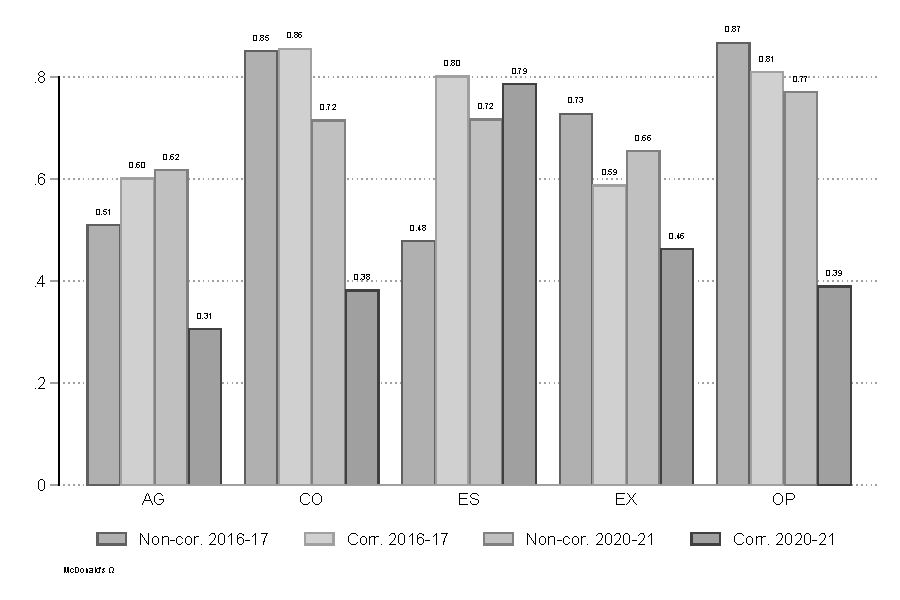
\includegraphics[scale=0.8]{INPUT/omega}
\caption{Internal consistency of Big-5 personality traits -- Distribution of \citeauthor{McDonald1999}'s $\Upomega$ through time and correction for 953 individuals in 2016-17 and 1,316 in 2020-21 from rural Tamil Nadu, India.}
\sourcefig{NEEMSIS-1 (2016-17) \& NEEMSIS-2 (2020-21); author's calculations.}
\label{fig:omega}
\end{figure}

%\paragraph{Factor analysis}
As warned by \cite{Laajaj2019}, the Big-Five taxonomy is limited in developing countries for several reasons: the enumerator-respondent interactions in face-to-face survey can induce a bias; the low education levels can make questions more difficult to understand and can induce a systematic response patterns, especially the acquiescence bias.
The very good knownledge of the field (see section \ref{subsection:data}) allow us to collect data of high quality and avoid a bias due to misunderstanding of questions.
Moreover, we implement our own factor analysis of the 35 questions by principal component with promax rotation.
To avoid a bias in factor analysis, we do not recoded reverse questions beause it might force likeness with Big-5 taxonomyIn our dataset, acquiesence bias is measure with a set of reverse questions that are supposed perfectly opposed to another set of questions. 
However, the assumption of opposition is supportable only in the Big-5 taxonomy, in another layout pairs of questions can measure different aspects of personality.
The resulting factors for 2016-17 data are relatively similar to the Big-5 personality traits with satisfactory \citeauthor{McDonald1999}'s $\Upomega$: Factor 1 as Openness-Extraversion ($\Upomega=0.91$); Factor 2 as Conscientiousness ($\Upomega=0.88$); Factor 3 as \textit{Porupillatavan} --tamil terms for talkative, easily distracted individual-- ($\Upomega=0.69$); Factor 4 as Emotional stability ($\Upomega=0.78$) and Factor 5 as Agreeableness ($\Upomega=0.62$) (see Appendix \ref{section:efa_big5}) while resulting factors for 2020-21 data are very different to the Big-5 taxonomy and to the 2016-17 factors\footnote{We do not present results here because we do not use it as personality traits measure, however it is available on request. See section \ref{subsection:econometricframework}.}.

%\paragraph{Life-cycle effects}
To mitigate against the potential problem of life-cycle events --that might induce endogeneity through measurement error-- [or to remove the effect of age on the \PTCS~ measures], we run univariate OLS regression with cognitive skills and personality traits as endogenous variables and age as exogenous variable. %(see Appendix \ref{section:efa_big5}).
We standardised the resulting residuals and use it at as age-effect-free \PTCS~ or net of life cycle influences \citep{Nyhus2005, Brown2014, Groves2005}. 

%\paragraph{Exogeneity}
The exogeneity of \PTCS~ is well assume because of stability over time while there is no consensus in psychology \citep{Ardelt2000, Deary2014}.
Our data allow us to examine stability over time of \PTCS~ for 835 individuals of rural India.

For personality traits, according to \cite{Costa1997, McCrae2000} it remains stable, in part, because it is a genetic predisposition that, by definition, cannot be changed over life.
Many economist\footnote{But not all, see \cite{Borghans2008, Almlund2011, Heckman2011}. As stated by \cite{Heckman2011}, ``Personality traits are not set in stone. They change over the life cycle. They are a possible avenue for intervention and policy.''} follow this path and the majority of then assume stability over time after the age of 25 and other verify this stability \citep{CobbClark2011}.
The stability refutes sociological and psychological literature which interesting in the influence of childhood and adulthood socialization on personality \citep{Mortimer1978, Moen1995}.
Following this path, \cite{Ardelt2000} state that ``personality can change over the course of a person's life, particularly if age at first measurement is low or over 50, if the retest interval is large, if individual personality aspects rather than the overall personality are considered, and if personality aspects other than the big five [...] traits are assessed.''
Our results show a stability for minor part of the population (see Appendix \ref{section:stab_big5}).
Non-corrected traits, in addition to having globally (2016-17 and 2020-21) higher internal consistency (see Table \ref{fig:omega}) are less unstable over time without being able to relate stability.

Concerning cognitive skills, majority of individuals have higher --or equal-- score in 2020-21 than in 2016-17 (see Appendix \ref{section:stab_big5}) which coroborate with the lifelong learning theory.
It is the continuing development of knowledge and skills that people experience after formal education and throughout their lives \citep{London2011}.



	% ******************************
	\subsection{Indebtedness measures}
	% ******************************

There is no consensus in the literature to measure indebtedness but three approaches are often retained.
Objective measures focus on the ability (or inability) to service or repay debts.
Typically, it is the debt to income ratio, debt to asset ratio, debt service ratio.
%Over-indebtedness occurs when a certain threshold is exceeded.
Although this is the most widely used measure, it under-estimate the burden of debt in ousting personal feeling and sacrifice associated with debt and over-indebtedness \citep{Betti2007}.
 
Subjectives measure assume that ``individual households are the best judges of their own net debt/wealth position'' \citep{Betti2007}.
The robustness of the results are based on the degree of honesty and literacy of individuals that can make it, sometimes, less reliable \citep{DAlessio2013}.
As stated by \cite{Rinaldi2006} and \cite{Keese2012}, in general, objective measures align quite well with subjective measures at the household classification level.

Last, administrative measures treat indebtedness  as ``all cases where non-payment of debts have been registered officially or declared before a court'' \citep{Betti2007}.
In rural Indian context, this type of measures have little meaning since most of the debt is informal.

% In order to best measure the debt, we could combine objective and subjective measures as \cite{Aniola2012} do in European Countries, but this brings the risk that all households will find themselves categorized as over-indebted according to the measure used \citep{Chichaibelu2018}.

It is recommended to analyse indebtedness at household level because generally income is grouped between household members \citep{European2010}.
However, in order to explore the role of individual characteristics such as \PTCS~ on indebtedness, we focus on two types of individual objective measures allowing us to understand the debt from three angles.
First, we investigate the size of the individual debt with the total amount of individual debt taken out in her own name.
Second, we investigate the burden of debt repayment with the individual debt service ratio (DSR).
It represent the share of income required to cover the repayment of interest and principal on a debt for one year.
We also complete the analysis with the probability for an individual to being in debt to capture the role of \PTCS~ on the incidence of debt.

% First, we wish to understand the role of personality traits \& cognitive skills on the incidence of individual debt --through the probability of being in debt\footnote{Dummy variable equal to 1 if the individual has some unsettled debt taken out in her own name, 0 otherwise.} in 2020-21.


	% ******************************
	\subsection{Econometric framework}
	\label{subsection:econometricframework}
	% ******************************

%\cite{Heckman1976}
In order to better understand the relationship, our analysis take place in three step.
\paragraph{How \PTCS~ shape individual debt?}
In a first step, we use the five factor of 2016-17 factor analysis as personality traits ($X'_{i}$) on individual debt of 2020-21 to understand how personality shapes individual debt.
Our analysis faces non-random sample selection issues because of the nature of our dependent variables: the sample is restricted to those who declared a non-zero and non-missing debt.
We therefore do not account for entry and exit in debt by only considering total loan amount and debt service ratio.
To overcome this sample selection issue, it is rigorous to use the Heckman procedure, which involves estimating a model of debt participation, where this is conditioned on factors additional to those that determine the amount of debt borrowed (exclusion restriction variables).
Strong theoretical background is needed to determine exclusion restriction variables that affect the participation decision but not the amount of debt.
\cite{Lennox2011} point out that an absence of exclusion restriction in the first stage can lead to severe multicollinearity in the second stage.
\cite{Cox1993} used years of education, occupation, area income, employment status and rural-urban status and \cite{Bertaut2002} used the proportion of household heads employed in the financial services in the region and the proportion of household heads employed in a workplace of 500 or more.
\cite{Duca1993} and \cite{Crook2001} assumed that the same variables determined the probability of having debt and the amount borrowed.
\cite{Rio2006} used localisation, race and employment status.
However, their results from Heckman procedure are no different from those from OLS regressions, suggested that ``any corner-solution biases are small''.
Therefore, they focus separatly on the participation equation and on debt equations (excluding non-participants).
We follow \cite{Rio2006} in focusing separatly on the participation equation and on debt equations in excluding non-participants.
\dev{Préciser que Indeed, nous aussi on a tenté un Heckman avec les var de la literature mais elles ne fonctionnent pas, il y en a qu'une qui fonctionne c'est debtor ratio, d'où le fait qu'on fasse comme Rio.}
We also estimate a Heckman selection model as robustness check with the household debt dependency ratios --defined as the number of indebtedness individuals divided by the total number of household members, in 2016-17-- as exclusion restriction variables.
We also check for multicollinearity and find that the highest VIF score is 4.33, which is less than the cutoff point of 10 \citep{Lennox2011}.
Results [available on request] are no different from those from OLS regression, suggested that the non-random sample selection issues is small, which coroborate with literature \citep{Rio2006, Brown2014}.
Another way to estimate our model is to use tobit model which allow for the truncation of the dependent variables as \cite{Brown2014, Cox1993}.
However, it would be unsuitable as the data are not censored or truncated, but defined on $\mathbb{R}^{+}$ \citep{Maddala1991}.


% We used t allowing to compute an inverse Mill’s ratio ($IMR_{i}$) to correct for non-random selection sample in our equations of interest (eq. \ref{eq:ols}).
% \par\noindent\rule{\textwidth}{0.4pt}
% \dev{Intuition:}
% Un ménage avec beaucoup d'individus endettés peut être le reflet d'un ménage dans le besoin.
% Afin de bénéficier quotidiennement des ressources nécessaires, sans pour autant que les individus aient à porter un lourd fardeau de la dette, une stratégie de "diversification des individus" peut être adoptée....!
% Les individus "devront" s'endetter afin d'apporter les ressources nécessaires au ménage, sans pour autant que les montants soient élevés.
% D'autre part, un ménage où beaucoup d'individus sont endettés, rend l'endettement "normal" aux yeux des autres membres.
% Dans notre contexte, les individus s'endettent pour survivre, il est normal de s'endetter.
% Donc j'ai tendance à croire que plus il y a des individus endettés dans le ménage, plus la pratique sera normal, d'autant plus que quasi tout le monde l'est dans le contexte, cependant, chacun s'endette à "son aise"..!
% Le niveau dépend plus des richesses de la famille, du travail, je pense...!
% Our IMR is less likely to be subject to this problem, because our first stage includes \dev{debtor ratio} and thus meets this restriction.
% To examine the robustness of our Heckman two-stage results, we first estimate eq. \ref{eq:ols} excluding IMR. 
% The coefficient on \PTCS are reported on Appendix, however, coefficient and t-stat are relatively similar.
% \par\noindent\rule{\textwidth}{0.4pt}


Therefore, we use, first, probit model with maximum likelihood estimation to estimate the probability for an individual of being in debt ($Indebt_{i}$) (eq. \ref{eq:probit}).

\begin{equation}\label{eq:probit}
\begin{split}
Indebt_{i}=\upbeta_{0}+X'_{i}*\upbeta_{1}+C'_{i}*\upbeta_{2}+Z'_{i}*\upbeta_{3}+\upmu_{i}
\end{split}
\end{equation}

Our control variables ($C'_{it}$) take the existing classic controls:
\begin{itemize}
\item Individual level variables as age; age square; sex; dummy variable which take 1 if individual is the household head, 0 otherwise; main occupation\footnote{Define as the most time-consuming activity.}; number of occupation (dummy variable which take 1 if individual declare more than one occupation, 0 otherwise); dummy variable which take 1 if individual received formal education through school, 0 otherwise (no formal education) and a dummy variable for marital status (1 if married, 0 otherwise). 
\item Household level variables as caste; monetary value of assets\footnote{The monetary value of assets includes gold; land; house; livestock; agricultural equipment and consumption good (car, computer, cookgas, phone, etc.).}; sex ratio; total annual income; household size; shock exposure (dummy variable which take 1 if the household experienced a shock\footnote{Marriage of at least one of the household members or/and household surveyed after the demonetisation.} between 2010 and 2016-17, 0 if not). 
\end{itemize}
The amount of debt is estimated in $t+1$ and our independent variables in $t$, we therefore control for the indebtedness situation in $t$ in adding dummy variable which take 1 if individual is indebted in 2016-17, 0 otherwise.

In order to investigate the amount of debt and the burden of repayment ($Y_{i}$), we use OLS (eq. \ref{eq:ols}).
Despite the fact that DSR is a share, we do not use GLM because of the upper bond of the variable ($>1$) \citep{Cook2008}.
\begin{equation}\label{eq:ols}
\begin{split}
Y_{i}=\upbeta_{0}+X'_{i}*\upbeta_{1}+C'_{i}*\upbeta_{2}+Z'_{i}*\upbeta_{3}+\upepsilon_i
\end{split}
\end{equation}

To take into account the strength of social identity we investigate relationship on a pooled sample of egos with interactions variables to maximize statistical power, although splitting samples improves model specification\footnote{The statistical power is not maximize if we use split samples.} .
First we do not use interaction to see the global effect (1), then we add interaction variable with sex (2), caste (3) and both (4) to test wether the effect of \PTCS~ differ by sex and caste:

\begin{table}[h!]
  \centering
    \begin{tabular}{lllll}
    (1)~~~~ $Z'_{i}=0$ & & & & (3)~~~~ $Z'_{i}=Caste*X'_{i}$ \\
    (2)~~~~ $Z'_{i}=Sex*X'_{i}$ & & & & (4)~~~~ $Z'_{i}=Sex*Caste*X'_{i}$ \\
    \end{tabular}%
\end{table}%

We choose to cluster the error at households level to take into account the fact that observations within each household are not i.i.d.
Indeed, we have data for two individuals from the same household and these latter sharing resources and pooling others.%\footnote{See \cite{Lazear1988} or \cite{Bonke2015} more recently.}.
In terms of debt, as stated by \cite{Reboul2021}, ``our data is limited, [but] it suggests that fully pooling and sharing the household debt burden is not the norm.''

To interpret our results, we compute marginal effect (ME) at representative values on the predicted values of \PTCS.%~ \cite{Williams2012}.
We use sex (male vs female) and caste (non-dalits --or middle-upper caste vs dalits) as representative values, all other variables are at mean.
Thanks to our interactions variables, we obtains nine groups of ME for each \PTCS~ variable: average individual; average male; average female; average non-dalits; average dalits; average non-dalits male; average dalits male; average middle-upper caste female and average dalits female. 

We use Big-5 taxonomy as robustness check.

\paragraph{How the \PTCS~ varies across the indebtedness distribution?}
As OLS regression is mean reasoning, we supplement this analysis with quantile reasoning to understand the variation of \PTCS~ across the indebtedness distribution.
Quantile debt regressions consider specific parts of the conditional distribution of the debt and indicate the influence of the \PTCS~ variables on conditional debt.
Therefore, we estimate eq. \ref{eq:ols} with quantile regression respectively at P10, P25, P50, P75 and P90 of the distribution.
Controls variables remain the same and we also cluster the error at households level.
To fully understand the results we do not use interaction variables ($Z'_{i}=0$) and we compute ME at means to investigate the relationship between debt and \PTCS~ for the average individual at specific percentile of the distribution.

\paragraph{How \PTCS~ influences the debt trajectory?}
In a third step, we try to understand the debt trajectory through time.
With a multinomial probit, we investigate the contribution of \PTCS~ on the debt trajectory: Never indebted in 2016-17 and 2020-21 (i); Out of debt between 2016-17 and 2020-21 (ii); Became indebted between 2016-17 and 2020-21 (iii); Always indebted in 2016-17 and 2020-21 (iv).

\begin{equation}\label{eq:mprobit}
\begin{split}
Trajectory_{i}=\upbeta_{0}+X'_{i}\upbeta_{1}+C'_{i}\upbeta_{2}+Z'_{i}*\upbeta_{3}+\upalpha_{i}
\end{split}
\end{equation}

We use the same vector of control variables than for the two previous approach, we also cluster the error at households level and we compute ME at representative values (sex and caste at representative values).
We also use Big-5 taxonomy as robustness check.

\paragraph{How does debt change over time as \PTCS~ changes?}
In a last step, we fully accept the non-stability of personality traits by using one-way\footnote{We choose to not compute two-way fixed effect for the many problems with maintaining assumptions and interpreting the coefficients \citep{Kropko2020,Imai2020}.} individual fixed effect regressions (eq. \ref{eq:fe}) in order to compare within individual over time.
In other words, as \PTCS~ increases for an individual over time, how does the debt change over time?
Unlike the previous approach, we do not use personality traits from factor analysis insofar as factor for 2016-17 are different from those for 2020-21.
The resulting factor from factor analysis of 2016-17 and 2020-21 are not interpreted in the same way, therefore, we cannot analyse the evolution of a given factor.
While the way we compute Big-5 personality traits allow us to analyse evolution because we use the same method in 2016-17 and 2020-21.
We use the same debt measures as before --the total amount of debt and the individual DSR-- as endogenous variables ($Y_{i}$). 

\begin{equation}\label{eq:fe}
\begin{split}
Y_{it}=X'_{it}\upbeta_{1}+C'_{it}\upbeta_{2}+Z'_{it}*\upbeta_{3}+\upalpha_{i}+u_{it}
\end{split}
\end{equation}

We use the same vector of control variables than before.
However, as we estimate FE model, time-invariant variables are omitted from the analysis: sex; education; caste. 
Cluster remains the same and ME at representative values (sex and caste) are computed.

An important caveat lies in the study of causality.
We do not pretend to show a causal relationshipt between \PTCS~ and indebtedness but to relate correlations because we cannot rule out the possibility of reverse causality between \PTCS~ variation and indebtedness variation.



%\newpage
% ***********************************
\section{Descriptive statistics}
% ***********************************

\subsection{Household unit in Table \ref{tab:descHH}}
Our final sample consists of 835 individuals from 473 households and almost half are dalits.
Three quarters of households have 2 egos, the last quarters have only one egos --justifying the fact that we cluster the error at household level.
The sex ratio is different through caste: in 24\% of dalits households the sex ratio is equal to 1 which mean that they are as many men as women while in middle-upper caste, it is 34\% of households in 2016-17.
In terms of assets, middle-upper caste households are three times richer than dalits on average --respectively 1,493k INR and 487k INR in 2016-17.
50\% of middle-upper caste have less than 666k INR of assets while 50\% of dalits households have less than 266k INR in 2016-17.
For 50\% of dalits, the monetary value of assets increased by at least 47\% between 2016-17 and 2020-21 while for 50\% of non-dalits households, it decreased by at least 22\%.
However, middle and upper caste still have higher amount of assets in 2020-21.
This economic advantage of non-dalit households is also found with income: the median income of middle-upper caste is 34\% higher than dalits one in 2016-17 and 15\% higher in 2020-21.
Last, whatever the caste, we observe a reduction of total income: for 50\% dalits households the total income decreased by at least 4\% and for 50\% of non-dalits households, it decreased by at least 5\%.
		
\subimport{INPUT}{desc_HH.tex}

\subsection{Individual unit in Table \ref{tab:descindiv}}
At egos level, 55\% of our sample are male and among them, 46\% are dalit (among female 50\% are dalit).
Male are, on average, older than female and three quarters of them are the head of household while female are only 9\% in 2016-17 and 27\% in 2020-21.
This increase is partly due to the life cycle: when the household head died, is the wife who takes over as household head.
In terms of education, male are more formal educated than female.

Disparities in terms of gender are also found in the occupation.
Despite the increasing of the number of female in agriculture and the decreasing of the number of male in self-employment, this activities are mostly reserved for male.
The reverse assessment is true for salaried job in agriculture: between 2016-17 and 2020-21 the share of male increase by 47\% (from 16\% to 24\%) but female remain relatively more numerous (27.42\% in 2016-17 and 29.58\% in 2020-21). 
Whatever the gender, non-agricultural salaried job remain stable over time and the share of male implicated is similar to the share of female (around 37\%).
Non-income generating work as the main occupation is over-represented for female while even though the share fell considerably between 2016-17 and 2020-21 (from 24\% to 15\%).
Moreover, female are more likely to have multiple occupations and this probability increase between 2016-17 and 2020-21 (from 50\% to 60\%).
In terms of income, disparities persist between male and female.
On average, male have 102,000 INR per year as labour income while female have 19,000 INR.
Between 2016-17 and 2020-21, the average variation rate is higher for female than for male (respectively 173\% and 163\%).

% \paragpraph{\PTCS}
Figure \ref{fig:PTCS} shows the distribution of each \PTCS~ net of life-cycle standardised.
Traits from Big-5 taxonomy (row 2) are not corrected from acquiesence bias.
The distribution of personality traits from Big-5 taxonomy and factor analysis seems to corroborate.
Indeed, in 2016-17, it appear that male tend to have higher score for each traits: they are more open to experience, conscientious, extraverted, agreeable and emotional stable.
When we compare 2016-17 distribution with 2020-21 one, we observe that, male --taken as a whole-- have slightly lower score for openess to experience and extraversion while female have slightly higher one.
Distribution of conscientiousness is more platikurtic and shifted to the right in 2016-17 than in 2020-21 for male: taken as a whole, male are less conscientious in 2020-21 than in 2016-17.
The assessment is reverse for female.
Distributions of agreeableness of 2020-21 are more platikurtic for male and female: taken as a whole, a more important share of male/female is very/less agreeable in 2020-21 than in 2016-17.
Conversely, distributions of 2020-21 for emotional stability are more leptokurtic for male and female.
Concerning cognitive skills, distributions of RPM are more shifted to the left in 2016-17 than in 2020-21: taken as a whole, a more important share of male/female have a low score at RPM in 2020-21 than in 2016-17.
For numeracy and literacy test, distributions are more shifted to the right in 2016-17 than in 2020-21: taken as a whole, a more important share of male/female have a high score in 2020-21 than in 2016-17.

% \paragraph{Individual debt trend}
There are many disparities in terms of debt.
While the share of individual is relatively stable through time and gender (around 75\%), the path is different.
Female are more vulnerable than male in the sense that the share of individual never in debt is lower for female than for male (respectively 10\% and 14\%) and the share of individual becomes in debt between 2016-17 and 2020-21 is higher for female than for male (respectively 14\% and 8\%).
To finish with the path, we observe that more than six out of ten individuals remains indebted.
Our sample of indebted individual consists of 643 individuals in 2016-17 and 606 individuals in 2020-21 whose 516 are indebted in 2016-17 and in 2020-21.
Male have a higher absolute amount of debt than female (two times more in 2016-17: 190,000 INR for male while 80,000 INR for female) despite a reduction in the amount between 2016-17 and 2020-21 (for 50\% of male, debt has decreased by more than 57\%).
On the other hand, 50\% of female saw their debt increased by more than 24\% (on average, in 2016-17 a female has a debt of 80,000 INR, while it is at 90,000 INR in 2020-21.
Male spend less of their annual income on debt repayment than female: in 2016-17 50\% of male spend 27\% of their annual income on debt repayment and 12\% in 2020-21 while female spend 32\% in 2016-17 and 77\% in 2020-21.
Furthermore, 50\% of male have seen their DSR decreased by at least 0.27\% while 50\% of female have seen their DSR increased by at least 0.09\%.


\subimport{INPUT}{desc_indiv.tex}

\begin{figure}[ht]
\raggedright
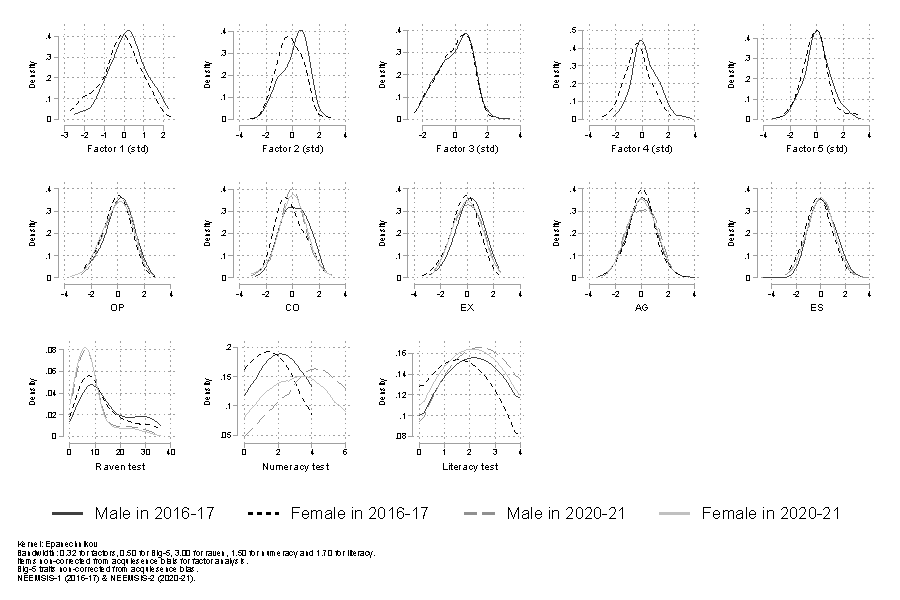
\includegraphics[width=\textwidth]{INPUT/Kernel_PTCS_raw_new}
\caption{Distribution of \PTCS~ -- The resulting \PTCS~ are based on the standardised residual from univariate OLS regression with age as exogenous variable. This is \PTCS~ purged from life-cycle effects.}
\sourcefig{NEEMSIS-1 (2016-17) \& NEEMSIS-2 (2020-21); author's calculations.}
\label{fig:PTCS}
\end{figure}



%\newpage
% ***********************************
\section{Results}
\label{section:results}
% ***********************************
%As stated by \cite{Amrhein2019, Wasserstein2019, Wasserstein2016} reported confidence interval

To interpret the results, marginal effects (ME) at representative values on the predicted value of the \PTCS~ are reported for the four specifications as describe previously.
According to specifications, the representatives values are: (1) the average individual (``All''); (2) the average male (``Male'') and the average female (``Female''); (3) the average non-dalits (``MUC'') and the average dalits (``Dalits''); (4) the average non-dalits male (``MUC male''), the average dalits male (``Dalits male''), the average non-dalits female (``MUC female'') and the average dalits female (``Dalits female'').
All of \PTCS~ are standardised to ensure comparability between them.
We will therefore speaks in terms of ``one standard deviation (sd)'' more of \PTCS.

An important caveat to acknowledge prior to exposing the findings of our empirical analysis is the magnitude of the effects.
They may seem high. 
However, this come from the low range of definitions of \PTCS~ variables.
For personality traits, ranging around from -4 to 4, one more \sd~ represent a gap of 1/8.
Put another way, for a variable ranging from -4 to 4, take an additional unit come back to take 12.5\% in more.

\subsection{How \PTCS~ shape individual debt?}
\paragraph{Probability of being indebted}
Table \ref{tab:ame_indebt} presents the results from the multivariates probit analysis of the probability for an individual to be indebtedness.
McFadden's pseudo $R^2$ indicate a very good goodness-of-fit for all the specification --they are all above 0.2 threshold \citep{McFadden1979}.
Moreover, we observe that all p-values associated with the simultaneous coefficient nullity test (LR $\upchi^2$) are low enough to conclude that at least one of the regression coefficients in the model is not equal to zero.
% and the exclusion restriction variable (Debtor ratio) is negatively correlated at the 95\% \cl. 

The results show that 2016-17 cognitive skill --whatever the specification-- are not correlated with the probability of being indebted in 2020-21 at 90-95\% \cl~(cl), except for literacy which is positively correlated for the average female.

However, three of the personality traits are correlated at the 95\% cl. 
Factor 1 as OP-EX is negatively correlated with the probability for the average middle-upper caste individual of being in debt and the relationship seems to be clarified for the average non-dalit female: \ote, when OP-EX increase by one \sd, the probability of being in debt decrease by 11.1 percentage point (pp).
The magnitude of the relationship is little less strong for Factor 3: when the average non-dalit female is one sd more \textit{Porupillatavan}, the probability of being in debt decrease by 8.4 pp, \aebe. 
Last, Factor 2 as CO is positively correlated (8.5 pp) for the average middle-upper male, \aebe.

If we accept a 10\% risk of error Factor 4 and 5 becomes correlated.
For the average dalit male, one more \sd~ on ES is associated by a decreasing of 6.2 pp of the probability of being in debt.
Regarding AG, it is negatively correlated for the average non-dalit individual and especially for the average non-dalit male.
The magnitude of the effect is lower than for CO (-6.7 pp compared to +8.5 pp).
Always for CO, at 90\% \cl, when it increase by one sd, the probability decrease by 7.7 pp for the average non-dalit female.

\subimport{INPUT}{AME_indebt.tex}


\paragraph{Total amount of debt}
Table \ref{tab:ame_loanamount} presents the results from the multivariates OLS analysis of the first outcome of the burden of debt, the total loan amount.
All p-values associated with the simultaneous coefficient nullity test (F-stat) are low enough to conclude that at least one of the regression coefficients in the model is not equal to zero.
The goodness-of-fit is less good than the previous one: we are able to explain around 23\% of the total variance of the total amount of debt.
% The IMR is insignificant across all four estimations \dev{(Be careful of three-way interaction)}, indicating that self-selection does not significantly affect total loan amount of debt after controlling for \PTCS and other controls variables.

Raven score is correlated with the total amount of debt at 95\% \cl~ for the average dalits female: \aebe, when Raven score increase by one \sd, predicted total loan amount increase by 21,000 \rupee.
At 90\% cl, numeracy is also correlated for the average dalits female, but positively and with lower magnitude (-16,000 \rupee).
Relationship between debt and Raven is reverse for the average non-dalit female with higher magnitude than for dalit female (+33,000 \rupee).

Regarding personality traits, Factor 1, 2 and 5 are correlated with the total amount of debt at 95\% \cl~ for, at least, one group.
For the average individual, OP-EX is positively correlated.
The relationship seems to be clarified for the average non-dalit individual and especially for the average non-dalit male for who one more sd in OP-EX is associated by a increasing of 49,000 \rupee~ of the total loan amount, \ote.
Always for the average middle-upper caste male, the strengh of the negative relationship is high enough (-64,000 \rupee) compared to other relationship. 
Last, AG is negatively correlated for the average dalits and especially for the average dalit female: when AG increase by one \sd, the total amount borrowed decrease by 15,000 \rupee.

At 90\% cl, new relationship appears for Factor 1 and 3.
When OP-EX increase by one \sd, predicted total amount borrowed increase by 13,000 \rupee~\ote, for the average dalits female.
Last, when the average individual is one sd more \textit{Porupillatavan}, the total loan amount decrease by 19,000 \rupee, \aebe.
The relationship is stronger for the average male (-24,000 \rupee) and for the average non-dalit individual (-29,000 \rupee).
 

\subimport{INPUT}{AME_loanamount.tex}

\paragraph{Individual debt service ratio}
Table \ref{tab:ame_idsr} presents the results for the individual debt service ratio.
All p-values associated with the simultaneous coefficient nullity test (F-stat) are low enough and the goodness-of-fit is quite low compared to previous analysis.
% The IMR is insignificant across all four estimations \dev{(Be careful of three-way interaction)}, indicating that self-selection does not significantly affect individual debt service ratio after controlling for \PTCS and other controls variables.

The results show that 2016-17 cognitive skill are not correlated with the total amount borrowed at 90-95\% \cl~.

As for the previous analysis, Factor 1 is positively correlated with the share of the annual income dedicated to debt (capital and interest) repayment and especially for average female and average dalits female at 95\% \cl.
Indeed, for the average dalit female, when OP-EX increase by one \sd~, the predicted DSR increase by 98 pp, \aebe.
CO is negatively correlated for the average individuals and the magnitude of the correlation is similar to that of Factor 1 (49 pp in more for OP-EX and 48 pp in less for CO, \ote).

\textit{Porupillatavan} and ES are correlated with the amount of debt if we accept a 10\% risk of error, especially for the average non-dalit female.
While the relationship is positive for Factor 3, the one with Factor 4 is negative and stronger (respectively +93,000 \rupee~and -136,000 \rupee).

\subimport{INPUT}{AME_IDSR.tex}



\subsection{How \PTCS~ varies across the indebtedness distribution?}

Table \ref{tab:ame_qreg} presents the results from the quantile regression on the total loan amount and DSR.

B=changement du dième décile de la distribution conditionnelle de la dette suite à une augmentation d'une unité de X.
Si binaire, B mesure l'écart entre le dième décile de la distribution conditionnelle de la dette des hommes et le dième décile de la distribution de la dette des femmes.




Loan amount 95 : literacy at p25 and ES at P50.
At 90\% cl, numeracy for P25 and P90.

DSR 95: OP-EX for P90
At 90\% cl, OP-EX for P75 and ES for P90.

%\subimport{INPUT}{AME_QREG.tex}

\begin{figure}[htpb]
\raggedright
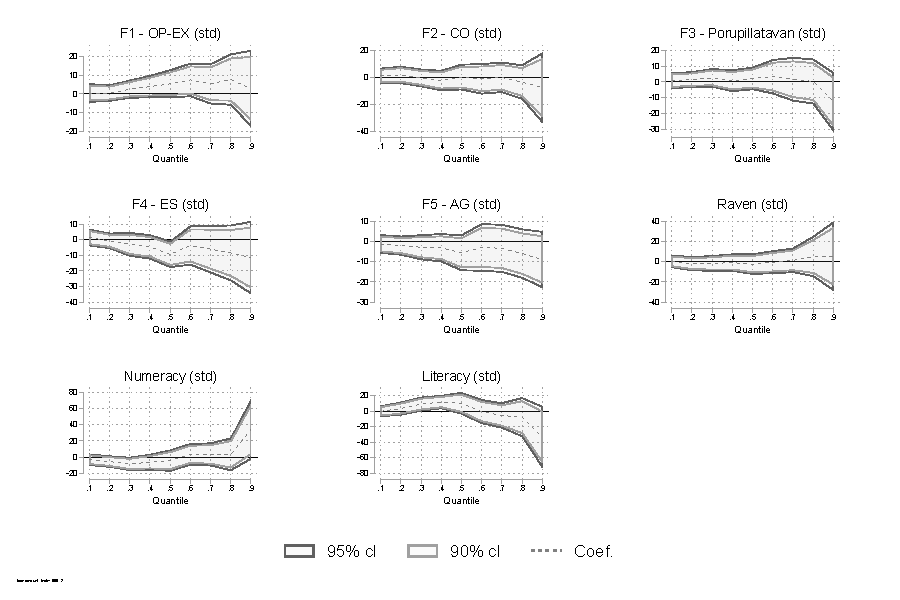
\includegraphics[width=\textwidth]{INPUT/qreg_loanamount_indiv1000_2}
\caption{Marginal effect on loanamount}
\sourcefig{NEEMSIS-1 (2016-17) \& NEEMSIS-2 (2020-21); author's calculations.}
\label{fig:qreg_loanamount}
\end{figure}

\begin{figure}[htpb]
\raggedright
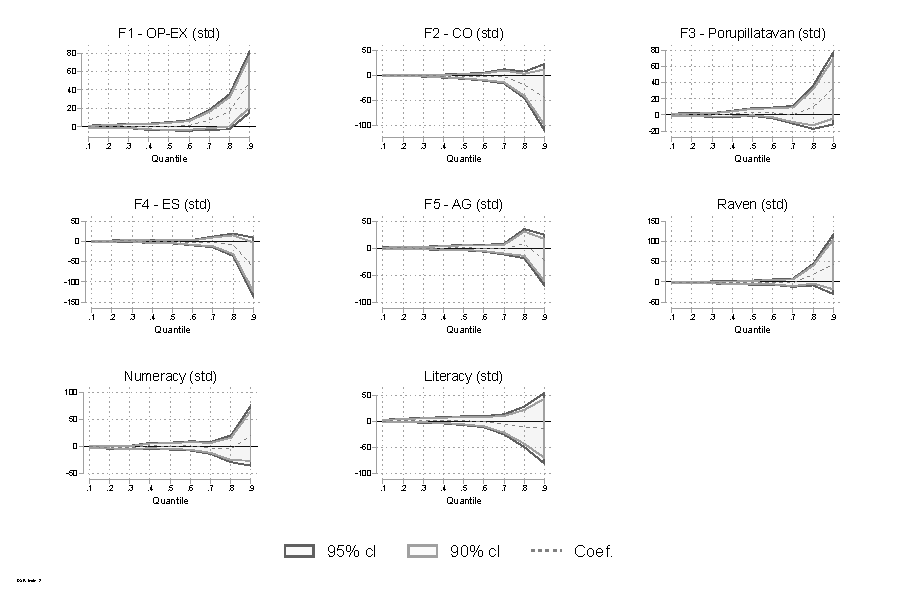
\includegraphics[width=\textwidth]{INPUT/qreg_DSR_indiv_2}
\caption{Marginal effect on DSR}
\sourcefig{NEEMSIS-1 (2016-17) \& NEEMSIS-2 (2020-21); author's calculations.}
\label{fig:qreg_dsr}
\end{figure}




\subsection{How \PTCS~ influences the debt trajectory?}
 Table \ref{tab:ame_debtpath} presents the results from the multinomial probit analysis of the debt trajectory through time.
 
\subimport{INPUT}{AME_debtpath.tex}



\subsection{How does debt change over time as \PTCS~ changes?}

\subimport{INPUT}{AME_FE_loanamount.tex}

\subimport{INPUT}{AME_FE_IDSR.tex}





\clearpage
\newpage
\section{Discussion and conclusion}

As argued in the introduction, the quantification of the role of \PTCS~ remains a blind spot of current debates about indebtedness.


This paper reveal a number of important insights.
Personality traits and cognitive skills are correlated with the probability of being in debt, the amount of debt and the burden of debt in rural India at different magnitude according to caste and sex.

% We discuss respectively our results with literature on \PTCS and debt (i); on social meaning of debt \citep{Guerin2014a, Guerin2020} (ii) and on \PTCS studies in India \citep{Michiels2021, Dasgupta2020, Gaurav2012, Donato2017} (iii).

\paragraph{\PTCS~ and debt in the literature}
Studies in northern countries reveal that emotional stability is a positive predictor of debt \citep{Nyhus2001}.
Our results seems to highlight reverse relationship with individual debt service ratio in rural India for non-dalits female (\citealp{Brown2014} find also relationship between neuroticism and debt for female).
For others groups, whatever the approach, we do not find significant relationship suggesting that this personality trait is not important in influencing level of debt, \aebe.
For non-dalits female given that emotional stability is related to pessimism, the finding that it has a negative association with individual debt is interesting in the context of the positive association found in the existing literature relating to financial optimism and debt.
Indeed, \dev{lit}.

Concerning openness and extraversion, \cite{Brown2014} find positive relationship with the probability of holding debt while our results suggest negative relationship for non-dalits female.
In terms of level of debt, we find that openness and extraversion are positively correlated with future debt which corroborate with \cite{Brown2014}.
When we interesting in the \PTCS~ variation on indebtedness variation, it appear that openness is positively correlated with the loan amount while extraversion is negatively correlated.
\dev{Why?}

Our findings on level of debt and burden of debt corroborate with \cite{Brown2014, Donnelly2012} who find that conscientiousness is inversely associated with the level of unsecured debt: individuals who are more conscientious are more able to ``manage their money through greater levels of financial self-control.''
Nevertheless, our results for non-dalits male are reverse to \cite{Nyhus2001, Brown2014}, who find that conscientious individuals are less likely to have ever been in debt.
\dev{Why?}



\cite{Brown2014}
\begin{itemize}
\item Small magnitude
\item For the probability of holding debt, CO inversely associated, les 4 autres positively
\item For relationship between finance and \PTCS~ accross debt distribution: in general there was no differential impact from personality traits on finances across the income distribution, the only exceptions being in the case of extraversion and neuroticism.
\item for gender : All other gender interactions with each personality trait are statistically insignificant.
\end{itemize}

\cite{Donnelly2012}
\begin{itemize}
\item For the probability of holding debt, CO inversely associated
\end{itemize}


\cite{Forlicz2019}
\begin{itemize}
\item 
\end{itemize}

\cite{Bertaut2002}
\begin{itemize}
\item 
\end{itemize}

\paragraph{Literature on individual debt practices}

\paragraph{\PTCS~ and other outcomes in rural India}

\paragraph{Conclusion}
As \cite{Brown2014} on montre l'importance des \PTCS~ dans l'analyse des finances


Numerous study reveal the gravity of the burden of debt for female and dalits, with double-jeopardy phenomenom. 
Here we highlight the fact that in this social identity, there is considerable differences.




% \newpage
% ***********************************
\section{Conclusion}
%\addcontentsline{toc}{section}{Conclusion}
\label{Conclusion}
% ***********************************

Malgré un double jeopardy avéré pour les dalits female, some tend to differenciate themselves with \PTCS~.
Les programmes de MC qui essayent de cibler les plus pauvres ne sont pas super efficient car même chez eux, il y a beaucoup de situation différentes en termes de dette.
Pose la question de l'inclusion financière


\clearpage
\newpage
%-------------------------------------------------------------------------------%
%\begin{nolinenumbers}
\addcontentsline{toc}{section}{References}
%\bibliography{C:/Users/Arnaud/Dropbox/Arnaud/Ref_Arnaud}
\bibliography{Ref_Arnaud}
%\nocite{*}



\newpage
%-------------------------------------------------------------------------------%
\appendix
\addcontentsline{toc}{section}{Appendix}



% \numberwithin{table}{section}
% \numberwithin{figure}{section}

%\section*{Appendix}
%\label{app:APP}


% ***********************************
% \section{Data description}
% \label{app:data}
% ***********************************

% In 2016-17, 492 households, 2,696 individuals, 953 egos.
% But, 2 households without egos.
% So we have 490 households and 953 egos.
% NEEMSIS2 (2020-21) recovered 485 households, 2,635 individuals.
% But, 600+1 individuals have left their households between the two wave, whose 98 egos.
% Which mean that we have 485 housholds and 2,034 individuals.
% But, we always have our two households without egos in 2016-17 that we can not compare.
% Thus, we have 483 households.
% But, for 10 households all egos have changed between 2016-17 and 2020-21.
% Egos of 2016-17 are still here in 2020-21, but they do not be selected as egos. 
% Finally, our sample is constitute from 835 egos represented 473 households.


%\clearpage
%\newpage
% ***********************************
\section{Stability of skills over time}
\label{section:stab_big5}
% ***********************************


% \begin{figure}[htpb]
% \raggedright
% 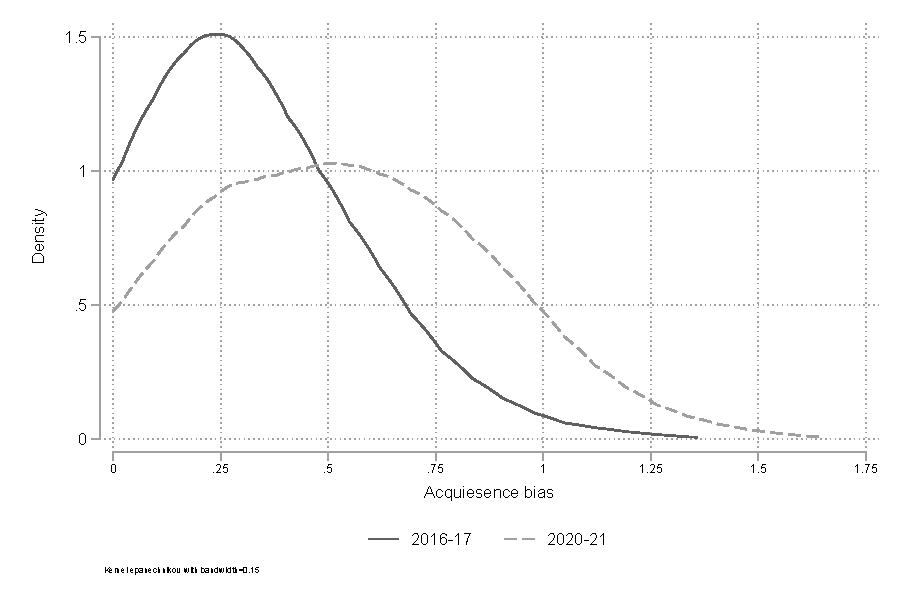
\includegraphics[scale=0.75]{INPUT/kernel_ars}
% \caption{Acquiescence biais in 2016-17 and in 2020-21 -- Distribution of acquiescence biais for 953 individuals in 2016-17 and 1,316 in 2020-21 from rural Tamil Nadu, India.}
% \sourcefig{NEEMSIS-1 (2016-17) \& NEEMSIS-2 (2020-21); author's calculations.}
% \label{fig:ars}
% \end{figure}

\begin{figure}[!htb]
\raggedright
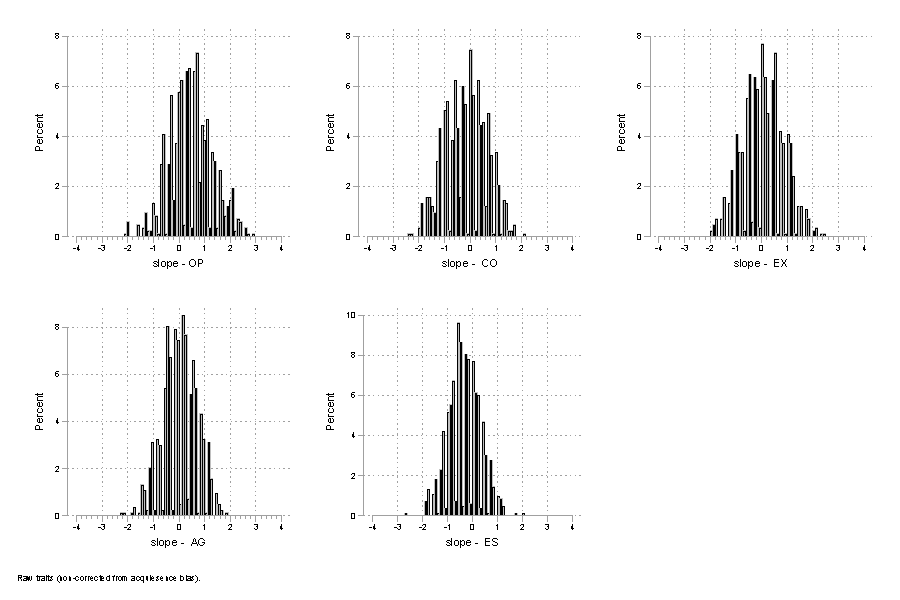
\includegraphics[scale=0.86]{INPUT/diffcont_raw}
\caption{Stability over time of Big-5 personality traits non-correted from acquiescence bias -- Distribution of the difference of the score between 2016-17 and 2020-21 for Big-5 personality traits non-corrected from acquiescence biais for 835 individuals from rural Tamil Nadu, India.}
\sourcefig{NEEMSIS-1 (2016-17) \& NEEMSIS-2 (2020-21); author's calculations.}
\label{fig:stabraw}
\end{figure}

\begin{figure}[!htb]
\raggedright
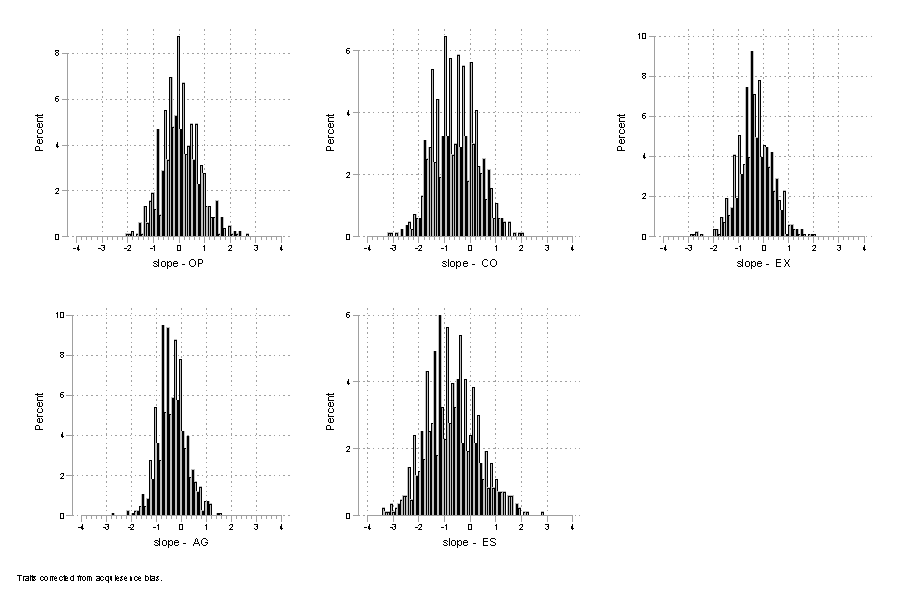
\includegraphics[scale=0.86]{INPUT/diffcont_cor}
\caption{Stability over time of Big-5 personality traits correted from acquiescence bias -- Distribution of the difference of the score between 2016-17 and 2020-21 for Big-5 personality traits corrected from acquiescence biais for 835 individuals from rural Tamil Nadu, India.}
\sourcefig{NEEMSIS-1 (2016-17) \& NEEMSIS-2 (2020-21); author's calculations.}
\label{fig:stabcor}
\end{figure}

\begin{figure}[!htb]
\raggedright
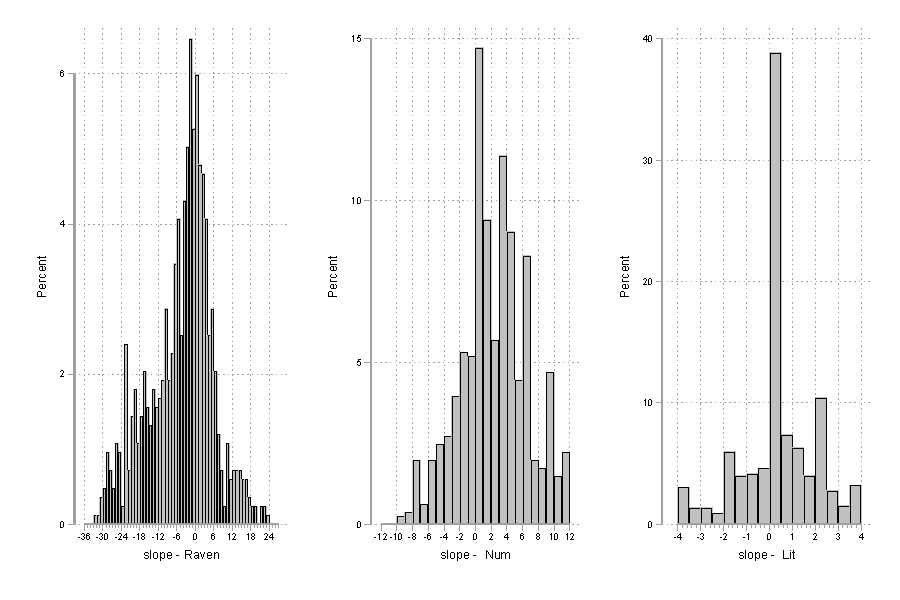
\includegraphics[scale=0.86]{INPUT/diffcont_cog}
\caption{Stability over time of cognitive skills -- Distribution of the difference of the score between 2016-17 and 2020-21 for three cognitive skills for 835 individuals from rural Tamil Nadu, India.}
\sourcefig{NEEMSIS-1 (2016-17) \& NEEMSIS-2 (2020-21); author's calculations.}
\label{fig:stabcog}
\end{figure}


\clearpage
\newpage
% ***********************************
\section{Factor analysis for personality traits}
\label{section:efa_big5}
% ***********************************


%\subimport{INPUT}{EFAres.tex}
\subimport{INPUT}{Big5.tex}

\clearpage
\begin{figure}[!htb]
\raggedright
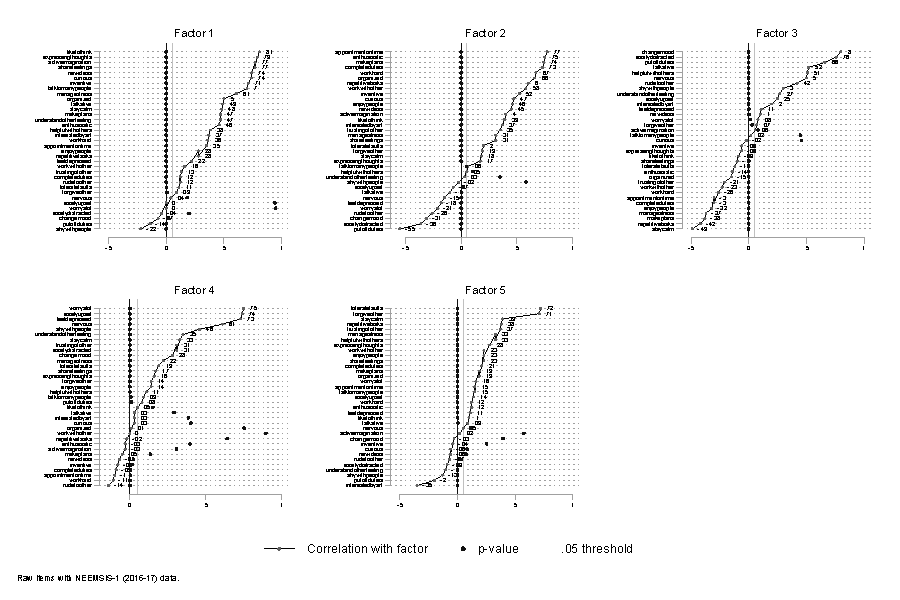
\includegraphics[width=\textwidth, angle=0]{INPUT/factor2016_2}
\caption{Results of factor analysis for 2016-17 raw items}
\sourcefig{NEEMSIS-1 (2016-17); author's calculations.}
\label{fig:resefa}
\end{figure}


\begin{figure}[!htb]
\raggedright
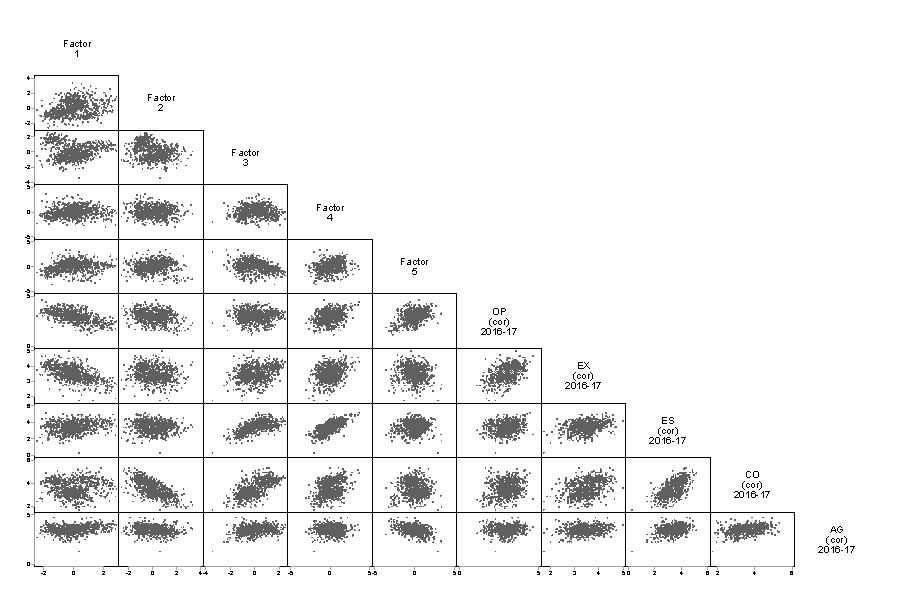
\includegraphics[scale=0.85]{INPUT/matrix_b5_efa}
\caption{Correlation between Factor from EFA and Big-5 personality traits}
\sourcefig{NEEMSIS-1 (2016-17); author's calculations.}
\label{fig:descXY}
\end{figure}




% \clearpage
% \newpage
% % ***********************************
% \section{Exclusion restriction variable}
% \label{app:imr}
% % ***********************************


% \subimport{INPUT}{imr_check_tab}

% \begin{figure}[!htb]
% \raggedright
% 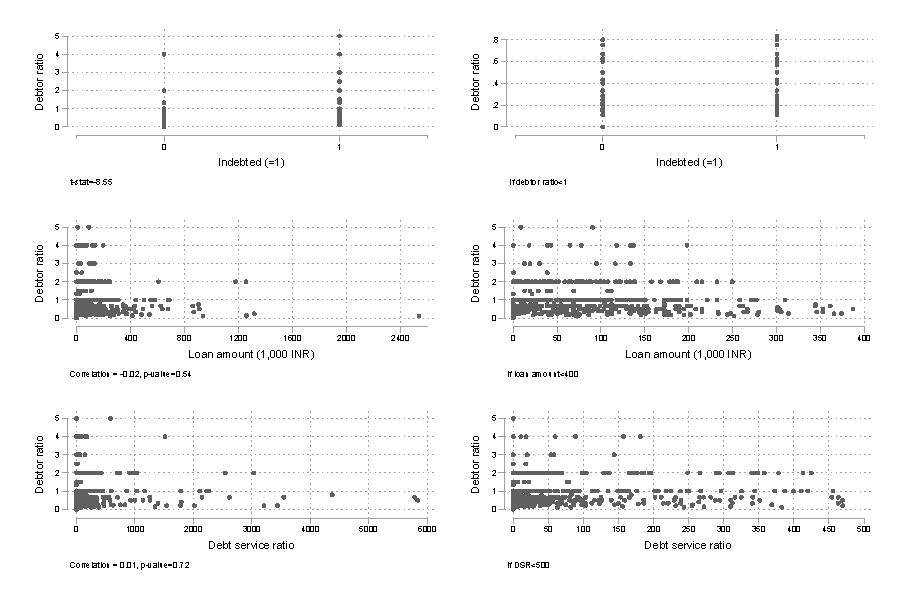
\includegraphics[scale=0.85]{INPUT/imr_check}
% \caption{Scatter plot and correlation test for IMR}
% \sourcefig{NEEMSIS-1 (2020-21); author's calculations.}
% \label{fig:imrcheck}
% \end{figure}


% \clearpage
% \newpage
% % ***********************************
% \section{Robustness check}
% \label{app:rob}
% % ***********************************

% \subimport{INPUT}{AME_indebt_b5.tex}
% \subimport{INPUT}{AME_loanamount_b5.tex}
% \subimport{INPUT}{AME_IDSR_b5.tex}
% \subimport{INPUT}{AME_debtpath_b5.tex}



% \clearpage
% \newpage
% % ***********************************
% \section{Detailed tables}
% \label{app:rob}
% % ***********************************
% \subimport{INPUT}{complet_indebt.tex}
% \clearpage
% \newpage
% \subimport{INPUT}{complet_fe.tex}
% \clearpage
% \newpage
% \subimport{INPUT}{complet_debtpath.tex}
% \clearpage
% \newpage
% \subimport{INPUT}{complet_indebt_b5.tex}



\clearpage
\newpage
%-------------------------------------------------------------------------------%
\setcounter{tocdepth}5
\tableofcontents

%\end{nolinenumbers}
\end{document}


%	% ******************************
%	\subsubsection{Social meaning of debt}
%	% ******************************
%\begin{itemize}
%\item Question de la confiance très présente dans la dette :
%\cite{Guerin2014a} Households’ creditworthiness is above all a matter of trust (nambikai), the term used locally
%when people refer to their ability to access credit. The fabric of trust covers many aspects that
%far exceed good credit history and repayment behaviour, and relates to every aspect of the
%borrowers’ reputation. Creditworthiness is rarely assessed on the individual level, and often
%incorporates the reputation and morality of the whole family or even lineage (Harriss-White
%and Colatei 2004). Lenders often state that they take two levels into account. One relates to
%family and lineage (taradaram), namely the family’s history, its “ethical” background and
%“morality”. The second level is individual (daram), relating very broadly to the “quality” of a
%person. It is therefore perfectly rational that the poor attach an equal importance to their
%reputation.
%
%“Behavior” also matters. As previously discussed, low castes are often seen as risky
%borrowers. Irrespective of caste, bad habits such as laziness, alcoholism and gambling are
%considered as indicators of poor repayment potential. As discussed above, respect and deference are also highly valued. Potential borrowers should equally show respect to their
%lenders and at times to its community.
%Giving money is a matter of respect. I respect them, they should respect me. How could I give them
%money if they talk badly about me? (Rajagopalan, Reddiar [FC], landowner and lender).
%If you don’t want credit from a particular community, then you can talk about them to others; otherwise
%you should not criticize. It might spoil creditworthiness. We should talk respectfully about these people,
%this is the only way to get creditworthiness (Gundusammy, Goundar (MBC), agriculture coolie and
%marginal farmer).
%
%\item Rapport de force
%\cite{Guerin2014}
%
%\citep{Guerin2020a}
%inseparable from an overall set of interdependencies, protection and social differentiation
%
%\item Social and moral experience
%imbued with subjectivities, felt-obligations and also aspirations
%
%\item Prestige sociale
%\cite{Guerin2014a}
%To understand debt practices, motivations and rationales, however, it is necessary to examine
%how the poor perceive and experience debt. It also requires taking into account the diversity
%of debt meanings and debt relationships. Of those in extremely vulnerable financial situations,
%very few consider themselves as over-indebted. The contrast between exogenous
%categorisations and local subjectivities is striking. One could of course argue that the poor
%suffer from “false consciousness”, in the sense that they are not even able to assess their own
%exploitation. Our explanation is different: we argue that the poor have their own “frameworks
%of calculations” (Villarreal 2009; this volume) and debt hierarchies (Shipton 2007). Such
%phenomena transcend questions of material or self-centred motivations and reflect issues of
%status, honour, power, and individual and group identity. This is our second argument:
%individuals engage multiple criteria to establish debt hierarchies and to evaluate debt burdens.
%Though financial criteria certainly matter, the social meaning of debt is equally, or more
%valued. While some debts are dishonoring, others are not. This depends upon the social
%relation between the debtor and the creditor and their respective status. Caste, class, kin and
%gender relationships are instrumental here.
%
%\cite{Guerin2014}
%Firstly, the social meaning of debt clearly matters. Debt is a marker of social hierarchy in
%kinship groups, the neighborhood and community alike. People try to avoid debts degrading
%to their status, or at least try to pay back these debts first.
%
%\end{itemize}
%
%
%\cite{Guerin2014a} : What is however clear is that over-indebtedness as a concept has little meaning to the poor.
%Financial indicators are certainly useful (and will be used here) to quantify the cost of debt.






% % ***********************************
% \subsection{Hypothesis}
% % ***********************************

% As we already note, the goal of this paper is to analyze the role of cognitive skills and personality traits on indebtedness in a context where \jati and gender conditionned individuals.


% firstly, check the contextual determinants of debt.
% Then, we add personality traits \& cognitive skills in the analysis to answer our first question: is cognitive skills and personality traits plays a significant role on indebtedness situation of households in rural India?
% Following literature, we can make H\ref{hyp:stability}.
% Indeed, concerning conscientiousness, \cite{Donnelly2012} state that ``highly conscientious individuals manage their money more because they have positive financial attitudes as well as a future orientation''.
% \cite{Brown2014, Nyhus2001} find similar results: conscientious individuals are less likely to have ever been in debt and conscientiousness is negatively related to the amount of unsecured debt.
% \cite{Nga2013} find that conscientiousness have a significant influence on risk aversion in Malaysia.
% \cite{Forlicz2019} find that for most of these countries there existed significant differences between debtors and debt-free individuals regarding the level of conscientiousness
% For neuroticism, \cite{Pinjisakikool2017b} find that emotional stability (inverse of neuroticism) significantly predict financial risk tolerance.

% \begin{hyp}[H\ref{hyp:stability}] \label{hyp:stability}
% Conscientiousness and neuroticism play significant role on household indebtedness [and over-indebtedness].
% \end{hyp}

% To understand the phenomenon more in depth, we decompose the analysis by caste, class and gender.
% The notion of class allow us to encompass ``property, wealth, occupation, income, and education'' \citep{Beteille2007}.
% We implement a multiple correspondance analysis with land property, wealth, occupation and income\footnote{We choose to not take into account education to stay at household level.} to create a dichotomy between high and low class (see appendix \ref{section:mca_class}).
% For caste and class decomposition, we formulate H\ref{hyp:poorer} imagining that cognitive skills are more important for lower households because we can imagine that higher one have all a high level of cognitive skills (math, literacy, etc.) because of better level of education\footnote{For the link between caste and education, see \cite{Borooah2005}.}.
% %\cite{Gaurav2012} find that cognitive skills significantly predict the financial aptitude and debt literacy for rural farmer in Gujarat
% %\cite{Agarwal2013} finds that ``consumers with higher math scores, are substantially less likely to make a financial mistake'' in separating our sample between economically and socially upper households and economically and socially lower households.
% \begin{hyp}[H\ref{hyp:poorer}] \label{hyp:poorer}
% Cognitive skills are better predictors for lower households than for higher one. 
% \end{hyp}

% Concerning gender, as \cite{Reboul2020} stated: ``[w]omen in the poorest households, despite meager incomes, have the highest borrowing responsibilities, shouldering the highest shares of household debt. [...] Their larger role in household debt management may be linked to their greater mobility and lower restrictions on social interactions, notably with men, which would underpin both their greater income shares and their access to credit relations. ''
% Thus, we can formulate the H\ref{hyp:women} hypothesis.
% \begin{hyp}[H\ref{hyp:women}] \label{hyp:women}
% When ego is a woman, her cognitive skills and personality traits play a bigger role in household finances than when ego is a man.
% \end{hyp}

% \cite{Reboul2019} Far beyond the issue of information about wages, the management of family finances leads
% to constant tensions and conflicts among family members, and thus gives rise to various tactics
% aimed at partially overcoming family constraints. This is particularly true for women, who have
% a heavy responsibility to ensure, among other things, daily expenses


% Last, we explore the source and use of debt in creating the dichotomy formal--informal and income generator--non-income generator of debt.
% Following results of \cite{Brown2014}, we formulate H\ref{hyp:filr}.
% \begin{hyp}[H\ref{hyp:filr}] \label{hyp:filr}
% Conscientiousness, extraversion, agreeableness and openess to experience have an association with informal debt.
% \end{hyp}

% To try to verify our hypotheses, we use original data set from rural south India.

% \cite{Guerin2014a} il faut aussi que je regarde le rôle des compétences cognitives sur la négociation de la dette en cross section : qui sont ceux qui arrivent le mieux à négocier leur dette ? 
% Comment savoir la negociation de la dette ? C'est le prix de la dette
% Prix de la dette p16 de \cite{Guerin2014a} The cost of \textit{terinjavanga} loans








% % ***********************************
% \section{Pistes en réflexions}
% % ***********************************

% \begin{itemize}[label=--]
% \item Quel est le score de l'\textit{homo oeconomicus} en termes de \textit{Big Five} ? \citep{Lopez2020}
% \item À partir de là, on peut chercher à voir si les autoentrepreneurs sont des \textit{homo oeconomicus} ou s'ils sont \textit{schumpeterien} ou \textit{coasien}.
% \item Analyse \textit{schumpeterienne} : \url{https://doi.org/10.4000/interventionseconomiques.1481}
% \item Regarder les articles de \cite{Gong2020} et de \cite{Srinivasan2005}
% \item Voir Occupational Attainment and Earnings in Southeast Asia: The Role of Non-cognitive Skills de Labour Economics, 2020
% \item salaire (y) = perso (x) -> OK; salaire (y) = perso (x) + educ (x) -> pas OK; perso passe par educ
% \item soulèvent; pointent; surlignent; mettent en évidence
% \item \cite{Yilmazer2005} + \cite{Poterba2001} + \cite{King1982}
% \end{itemize}





%---------------------------------
%KEEP THAT BUT NOT IN THE ARTICLE
%---------------------------------
%\paragraph{Retirement assets}
%Compared to China, the retirement pensions are not very efficient.
%Indeed, around 90\% of labor is informal [in the sense of absence of social insurance] and 85\% of non-agricultural workforce is informal \citep{Mehrotra2019}.
%For \cite{Badarinza2016b}, India figures as an outlier among low-middle-income countries on this point.
%\paragraph{Gold}
%\begin{itemize}
%\item On average, gold represent more than 11\% of indien household balance sheet  while it is less than 1\% in China \citep{Badarinza2016b}.
%\item Préciser les différences rurales urbaines de \cite{Badarinza2016b}.
%\item Mais rester sur le fait qu'au TN l'or est la première forme d'épargne d'après \cite{Roesch2008} \cite{Guerin2012a}
%\item Pourquoi ils aiment tant ?
%\item[1] Real estate has lower liquidity when compared with gold, and if liquidity needs are correlated with inflation volatility, gold better serves the purpose than real estate. Gold as a non-financial asset also has additional properties that are not provided for by real estate, such as a high collateral value and physical verifiability \citep{Badarinza2016b}
%\item[2] Avec la littérature d'Isabelle, parler du social role de l'or en rural India.
%\end{itemize}
%---------------------------------






% Mesure overindebtedness
% \item \citep{European2010} ont 5 recommendations pour bien mesurer:
% \item[1] Le surendettement s’analyse au niveau du ménage car les revenus des individus sont généralement regroupés ;
% \item[2] Les indicateurs doivent couvrir tous les aspects des engagements financiers : le logement, le crédit à la consommation, les factures, les emprunts hypothécaires ;
% \item[3] Le surendettement est considéré comme un état structurel car il implique une incapacité à faire face à des dépenses récurrentes ;
% \item[4] Le surendettement ne se résout pas en empruntant davantage ;
% \item[5] Pour qu’un ménage respecte ses engagements, il doit réduire considérablement ses dépenses ou trouver un moyen d’accroître ses revenus.




%\cite{John1999} the Big 5 "represent personality at the broadest level of abstraction, and each dimension summarizes a large number of distinct, more specific personality characteristics".






% FE
%For example, with regard to the question of whether \PTCS of individuals affects the debt of that individuals, we can investigate:
%\begin{itemize}
%\item Individual over time; 
%\item Cross-section of individuals in 2016-17 or 2020-21.
%\end{itemize} 
%If we look only at the time series for $HHINDID\_panel=KOR20/1$, we ask:
%\textit{As \PTCS increases for $KOR20/1$ over time, how does the debt change over time?}
%If we use one-way case FE, we generalize this question across individuals:
%\textit{As \PTCS increases for an individual over time, how does the debt change over time?}
%If instead we look at the cross-section that exists in 2016-17, we ask:
%\textit{How much more democratic are wealthier countries than poorer countries in 1990?}
%One-way time FE generalize this question to the entire time frame under analysis, and simply ask: 
%\textit{How much more democratic are wealthier countries than poorer countries at any point in time?}
%If a researcher intends to compare one case to itself over time, it is appropriate to examine individual time series and to use one-way case FE; if a researcher intends to compare one case to another at the same point in time, it is appropriate to examine cross-sections and to use one-way time FE. 
%If a researcher wishes to allow different cases to experience different over-time effects, or to let different cross-sectional effects exist at different points in time, it is straightforward to use interactions to extend a one-way FE specification to account for the desired heterogeneity \citep{Kropko2020}.





% Following \cite{Frank2000} and \cite{Larcker2010}, we next assess how closely an unobservable confounding variable would have to be correlated with DEBT and \PTCS~ to change the OLS results. 
% The Impact Threshold for a Confounding Variable (ITCV) is 0.116. 
% To put this number in perspective, the highest ITCV based on our identified control variables is 0.018 (for FINANCIALLY CHALLENGED). 
% This suggests that we would need an omitted variable with an impact of more than six times that of any of our control variables to change our results.
% Thus, there is unlikely to be a confounding variable that will overturn the positive association between ABSERROR and MW.
% \cite{Feng2009}